%%
%% This is file `example.tex',
%% generated with the docstrip utility.
%%
%% This is a file for illustrating the possibilities of LaTeX Beamer and the 
%% new IES beamer layout
%% 
%% Copyright (C) 2008 by Marco Huber <marco.huber@ira.uka.de>
%% 
%% This file may be distributed and/or modified under the conditions of
%% the LaTeX Project Public License, either version 1.2 of this license
%% or (at your option) any later version.  The latest version of this
%% license is in:
%% 
%%    http://www.latex-project.org/lppl.txt
%% 
%% and version 1.2 or later is part of all distributions of LaTeX version
%% 1999/12/01 or later.
%%
%
%
%\documentclass[english, 10pt,
%	final, %
%	% draft, % Grafische Elemente durch graue Boxen ersetzen (beschleunigt Kompilieren)
%	% 8pt, % Zu klein, erfordert Paket extsize
%	% 9pt, % Zu klein, erfordert Paket extsize
%	% 10pt, % f�r Folien mit sehr viel Text
%	% 11pt, % Standardschriftgr��e
%	% 12pt, % etwas gr��er und daher besser zu lesen
%	% 14pt, % deutlich gr��er, erfordert Paket extsize
%	% 17pt, % PowerPoint Standardschriftgr��e, erfordert Paket extsize
%	% 20pt, % sehr gro�, erfordert Paket extsize
%	% trans,% Zum Erstellen von Overhead Folien
%	% handout, % Erstellen eines Handouts (!)
%	% article,% Erstellen eines Artikels
% 	% compress, % Die Navigation in der Kopfzeile wird komprimiert dargestellt
%	%t, % Place text of slides at the (vertical) top of the slides
%	% c, % Place text of slides at the (vertical) center of the slides
%	% color={}, % list of options for color
%	%xcolor={table,dvipsnames}, % Optionen f�r xcolor �bergeben
%	% hyperref={bookmarksopenlevel=4}, % list of options for hyperref
% % %%%for bookmarks, the package bookmark can be used now!
%	% envcountsect, % Causes theorems, definitions, and so on to be numbered locally to each section.
%	% notheorems, % Switches off the definition of default blocks like theorem
%	% noamsthm, % Does not load amsthm and also not amsmath
%	% ucs, % lädt ucs Paket
%	% utf8, % lädt utf8x Paket von ucs (utf8 enconding)
%	% dvips, % erzwingt das Laden des dvips Treibers - idR nicht nötig!
%	% usepdftitle=false, % Suppresses the automatic generation of title and author entries in the pdf document information.
%	% ignorenonframetext, % suppresses content created for the article mode ??
%	%show notes, % enables Notes
%	% leqno,
%	% fleqn,
%]{beamer}
\documentclass[english, 10pt]{beamer}
%\documentclass[english, 10pt, draft]{beamer}
%\documentclass[english, 10pt, show notes]{beamer}
%\documentclass[english, 10pt, trans]{beamer}
%\documentclass[english, 10pt, handout]{beamer}

% Aktiviere die Sprachunterst�tzung und evtl. auch die Sprache:
% Die Sprache kann auch sp�ter mit Hilfe der Variable
% UseTranslation neu gesetzt werden

\usepackage{graphicx}
\usepackage{media9}

%%
%% This file enables creation of several versions
%% of a document with different lanuages
%% Copyright (C) 2008 by Michael Grinberg <mig@ira.uka.de>
%% 
%% Usage:
%%
%% 1. include this file with
%%      input{multilang}
%%
%% 2. Define your default language (first or second) with
%%      \setboolean{UseTranslation}{false} %use first language (=original)
%%    or
%%      \setboolean{UseTranslation}{true} %use second language (=translation)
%%    (!) You may reset this value if needed inside of your document
%%
%% 3. Whenever you need to have too versions of a text use
%%    \transl{Text in first language}{Text in zweiter Sprache}
%%


\usepackage{ifthen}


% boolean for defining translation use
%      true:  use the second language (= Translation)
%      false: use the first language
\newboolean{UseTranslation}
\setboolean{UseTranslation}{false}%Default: false. can be redefined in the text.




%\newcommand{\transl}[2][\relax]{%
%  \ifx#1\relax
%    #2
%  \else
%    \ifthenelse{\boolean{UseTranslation}}{#2}{#1}
%  \fi}



% Command dealing with several versions of text
\DeclareRobustCommand\transl[2]{\ifthenelse{\boolean{UseTranslation}}{#2}{#1}}

% F�r die Verwendung im Zwei-Bildschirme-Modus
% (s.PDF-Anleitung f�r Beamer-Class von Till Tantau)
% http://www.ctan.org/tex-archive/macros/latex/contrib/beamer/doc/beameruserguide.pdf
%\DeclareRobustCommand\transl[2]{\alt<second>{#2}{#1}}


% Setze Sprache:
% (Diese Variable kann je nach bedarf sp�ter neu gesetzt werden):
\setboolean{UseTranslation}{true}%Deutsch
%\setboolean{UseTranslation}{false}%Englisch


%for using two screens:
%\usepackage{pgfpages}
%
%\setbeameroption{second mode text on second screen=<location>}
%The <location> of the second screen can be left, right, bottom, or top.
%\setbeameroption{second mode text on second screen=right}

\newcommand{\hmmax}{0}
\newcommand{\bmmax}{1}

% Set depth of the Table of Content (=>depth of the PDFbookmarks)
% for better navigation
\setcounter{tocdepth}{4} 
% So tut es irgendwie nicht:

% Hier werden die verwendeten Pakete definiert
\usepackage[english, ngerman]{babel}
\usepackage[latin1]{inputenc}
\usepackage{array}
\usepackage{multicol}
\usepackage[absolute,overlay]{textpos}
\usepackage[babel]{csquotes}

\usepackage{multimedia}

\usepackage[final]{pdfpages}	%final: Inserts pages. This is the default.
										%draft: Does not insert pages, but prints a box and the filename instead.
										%enable-survey: Activates survey functionalities.
										%               (experimental, subject to change)

\usepackage[open, openlevel=3]{bookmark}

\usepackage{tikz}

%Einbindung zu verwendender TikZ-Bibliotheken
%(in diesem Beispiel werden eigentlich nur die Bibliotheken
%shapes.misc und decorations.pathmorphing verwendet)
\usetikzlibrary{calc,arrows,positioning,shadows,backgrounds,chains,topaths,matrix,scopes,decorations,decorations.pathmorphing,decorations.markings,fadings,shapes.geometric,shapes.multipart,shapes.misc,through,automata,fit}

% Definition eines TikZ Objekt: sehr dicker, schwarzer Pfeil, mit Pfeilspitzentyp 'stealth'
\tikzstyle{lblock}=[ultra thick, -stealth, black]


% Pfade f�r Videos und Bilder setzen
% Dies ist daf�r gemacht

% Verwendete Pfade: (Reihenfolge wichtig, da Durchsuchen in dieser Reihenfolge erfolgt!!!)
% Achtung: Es gibt keine Warnung, falls Pfade an mehreren Stellen gesetzt werden!
\graphicspath{{../Images/}{../Images/Grundlagen/}}
%
% Grafik-Erweiterungen
\DeclareGraphicsExtensions{.pdf,.png,.jpg,.jpeg,.bmp}


\newcommand{\videopath}{../Videos/}


% Das zu verwendete Design-Schema:
%\usepackage{PreambleFiles/KITdefs}
\usepackage{PreambleFiles/beamerthemeKIT}
%alter Aufruf:
%\usetheme{KIT}

% Please choose the correct outer theme for your slides:
% Die "outer theme", wo u.a. Logo-Platzierung und
% Gestaltung der Titelseite passiert, kann in der
% Datei beamerouterthemeXXXX.sty gesetzt werden
%
%\usepackage{PreambleFiles/beamerouterthemeIOSB}
%\usepackage{PreambleFiles/beamerouterthemeKIT-IES}
%\usepackage{PreambleFiles/beamerouterthemeIES-KIT}
%\usepackage{PreambleFiles/beamerouterthemeKIT-IOSB}
%\usepackage{PreambleFiles/beamerouterthemeIOSB-KIT}
\usepackage{PreambleFiles/beamerouterthemeIOSB-IES}
%\usepackage{PreambleFiles/beamerouterthemeIES-IOSB}
%


%\setbeamercovered{transparent}
%\setbeamercovered{invisible}
\setbeamercovered{
	still covered={\opaqueness<1->{0}},
%{	\opaqueness<1>{60}
%	\opaqueness<2->{30}},
	again covered={\opaqueness<1->{15}}
}

%possible templates are triangle, circle, square, ball.
%\setbeamertemplate{enumerate items}[ball]
\setbeamertemplate{itemize item}[ball]
\setbeamertemplate{itemize subitem}[triangle]
\setbeamertemplate{itemize subsubitem}[triangle]%[square]%
\setbeamertemplate{subsection in toc}[ball]%[ball unnumbered]%[circle]%[triangle]%[square]%
%\setbeamertemplate{subsection in toc}[subsections numbered]




%\usenavigationsymbols
%\usenavigationsymbols[sfHhdb]
%\usenavigationsymbols[sfhHb]

% Angaben zum Titel, Titelabbildung, Author und Institution




%-------------------------------------------------------
% Title
%-------------------------------------------------------
% Zwei versionen: Deutsche und Englische
\transl{%
%Title is made as a hyperlink for a fast navigation to the outline slide 
\title[\hyperlink{Outline}{CNNs}]{Implementation and Evaluation\\ of Extensions for CNNs}
}{%
\title[\hyperlink{Outline}{Logo Retrieval}]{Logo Retrieval in Massendaten mittels Deep-Learning}
}


%-------------------------------------------------------
% Title Graphic
%-------------------------------------------------------
%
%\titlegraphic{}
%\titlegraphic{\pgfuseimage{titlegraphic}}
%
\titlegraphic{%
\centering\centerline{\ifpdf{%
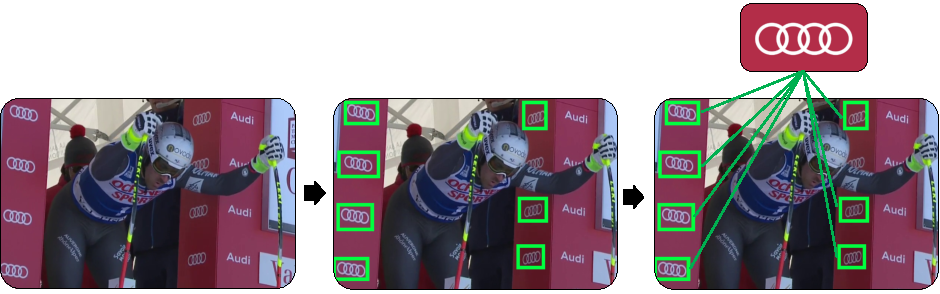
\includegraphics[height=14.5ex]{main}%
}\fi}%
}


%-------------------------------------------------------
% Author(s) / Presenter
% In eckigen Klammern Kurzversion für die Fusszeile
% (als Hyperlink zur Gliederung)
%-------------------------------------------------------
%
%
\author[\hyperlink{Outline}{Andras T\"uzk\"o}]{\textcolor{blue}{Andras T\"uzk\"o}}




%-------------------------------------------------------
% Date
% usage:   \date[short date]{date}
% Example: \date{\today} or \date[STACS 2003]{STACS Conference, 2003}.
%-------------------------------------------------------
%
\date{23. Juni 2017}


%-------------------------------------------------------
% Subtitle
%-------------------------------------------------------
%
\subtitle{Masterarbeit Abschlusspr\"asentation am \insertdate}
%\subtitle{Gespräch BAF am 29.06.2011}





%-------------------------------------------------------
% Institution(s)
%-------------------------------------------------------
%
\institute{\transl{%
%
%--------------------------------
% -   Hier englische Version    -
%--------------------------------
%
Karlsruhe Institute of Technology (KIT)\\
Institute for Anthropomatics\\
Vision and Fusion Lab (IES)
\\[2ex]
in cooperation with
\\[2ex]
Fraunhofer Institute of Optronics, System Technologies and Image Exploitation (IOSB)\\
Department Video Exploitation Systems\\
Karlsruhe, Germany%
%
%
}{%
%
%--------------------------------
% -    Hier deutsche Version    -
%--------------------------------
%
Karlsruher Institut f\"ur Technologie (KIT)\\
Institut f\"ur Anthropomatik\\
Lehrstuhl f\"ur Interaktive Echtzeitsysteme (IES)
\\[2ex]
in Kooperation mit
\\[2ex]
Fraunhofer-Institut f\"ur Optronik, Systemtechnik und Bildauswertung (IOSB)\\
\bigbreak
\small{\textbf{Betreuer:} Dipl.-Inform. Christian Herrmann, Dipl.-Inform. Daniel Manger}
}%transl
}%institute





%Hilfsmakros (Werden von Hauptmakros in Macros.tex verwendet):


%TODO-Gestaltungsmakro f�r Textmodus mit einer Unterscheidung, ob etwas �bergeben worden ist oder nicht
\newcommand{\myTodo}[1]{%
		\ifx\relax#1\relax% Falls Argument #1 leer:
			\textcolor{red}{\textbf{ToDo!}}%
		\else% Falls #1 mit Inhalt:
			\textcolor{red}{\textbf{ToDo:} #1}%
		\fi%
}

%TODO-Gestaltungsmakro f�r Mathe-Modus mit einer Unterscheidung, ob etwas �bergeben worden ist oder nicht
\newcommand{\myMathTodo}[1]{%
		\ifx\relax#1\relax% Falls Argument #1 leer:
			\textcolor{red}{\mathbf{\textnormal{ ToDo! }}}%
		\else% Falls #1 mit Inhalt:
			\textcolor{red}{#1}%
			%\textcolor{red}{\mathbf{\textnormal{ ToDo: }}{#1}}%
		\fi%
}



%[#1]: optional: Pfad zu einem bereits vorhandenem Bild, das �berarbeitet werden soll (in eckigen Klammern)
%{#2}: TODO-Beschreibung
\newcommand{\myImgTodo}[2][]
{
 % new figure floating environment
 \begin{figure}[!htb]
  \centering
  % TODO-image
		\ifx\relax#1\relax%
			\begin{tikzpicture}
				\draw[
					use as bounding box,
					black,
					thick,
					double, 
					double distance = 4pt, 
					rounded corners = 6pt] 
					(-4,-3)rectangle(4,3);
					\node[rotate=45,scale = 5,opacity = 0.5] at (0,0) {TODO!};
			\end{tikzpicture}
		\else%
			\includegraphics[width = 0.8\textwidth]{#1}\relax
		\fi
	\caption{\myTodo{#2}}
 \end{figure}
}

% -- new commands by MiG---

%Achtung! Diese Datei verwendet Hilfsmakros aus der Datei AuxiliaryMacros.tex!


%1.) Befehle zum Rumspielen mit Layout:

%Optionale Herleitungen, die bei Bedarf ausgelassen werden k�nnen:
%\newcommand{\reduce}[1]{\relax} % --> Optionale Herleitungen reduzieren
\newcommand{\reduce}[1]{#1} % --> Optionale Herleitungen nicht reduzieren

\newcommand{\code}[1]{\textsf{#1}}

%Befehl zum Hervorheben wichtiger Begriffe
%\newcommand{\mydef}[1]{\emph{#1}} %kursiv
%\newcommand{\mydef}[1]{\textbf{#1}} % fett
\newcommand{\mydef}[1]{\emph{\textbf{#1}}} %fett und kursiv

\newcommand{\rem}[1]{}  %Zum einf�gen von Kommentaren mitten in einer Zeile
%\newenvironment{rem}[1]{}{} %Blockkommentare funktionieren nicht, falls } mittendrin. 
% Verwende Umgebung {comment} aus dem entsprechendem Packet

%TODO-Befehle f�r den Textmodus
\newcommand{\todo}[1]{\myTodo{#1}} %\addToTodoList{#1}}
\newcommand{\ToDo}[1]{\todo{#1}}
\newcommand{\Todo}[1]{\todo{#1}}
\newcommand{\TODO}[1]{\todo{#1}}

%TODO-Befehle f�r den Mathe-Modus
\newcommand{\mathtodo}[1]{\myMathTodo{#1}} %\addToTodoList{$#1$}}
\newcommand{\mathToDo}[1]{\mathtodo{#1}}
\newcommand{\mathTodo}[1]{\mathtodo{#1}}
\newcommand{\mathTODO}[1]{\mathtodo{#1}}

%Erzeugen eines TODO-Bildes:
%[#1]: optional: Pfad zu einem bereits vorhandenen Bild, das �berarbeitet werden soll (in eckigen Klammern)
%{#2}: TODO-Beschreibung
\newcommand{\imgtodo}[2][]{\myImgTodo[#1]{#2}}
\newcommand{\imgToDo}[2][]{\myImgTodo[#1]{#2}}
\newcommand{\imgTodo}[2][]{\myImgTodo[#1]{#2}}
\newcommand{\imgTODO}[2][]{\myImgTodo[#1]{#2}}


%Add a ToDo without showing the TODO text in the document
\newcommand{\remtodo}[1]{\textcolor{red}{\textbf{ToDo!}}} %\addToTodoList{ToDo!}}


\newcommand<>{\mathred}[1]{{\color#2{red}#1}}
\newcommand<>{\mathblue}[1]{{\color#2{blue}#1}}


%-------------------------------------------------------
\begin{document}


%\setlength\textheight{71mm}
%\setlength\textheight{60mm}%{81mm}%{7cm}				% required for correct vertical alignment, if [t] is not used as documentclass parameter
%\setlength\textwidth{125mm}
%\setlength\textwidth{112mm}

%reset the inner spacing of the fbox
\setlength{\fboxsep}{0pt}




%-------------------------------------------------------
% Title Frame
%-------------------------------------------------------
%Only for the pdf bookmarks (for better navigation)
\transl{%
\part{Main Content}}{
\part{Hauptinhalt}}
%
\label{Titelfolie}
\transl{
\bookmark[level=2, dest=Titelfolie]{Title slide}}{
\bookmark[level=2, dest=Titelfolie]{Titelfolie}}
%------------------------------
\begin{frame}[c]
  \maketitle
\end{frame}
%------------------------------


%-------------------------------------------------------

\label{Motivation}

%Lesezeichen, die nicht in dem Inhaltsverzeichnis vorkommen sollen:
\bookmark[level=2, dest=Motivation]{Motivation}

%\input{Frames/Motivationsbild}

%-------------------------------------------------------
% Automatic Outline
%-------------------------------------------------------
%Only for the pdf bookmarks (for better navigation)
%
\transl{%
\bookmark[level=2, dest=Outline]{Outline}}{%
\bookmark[level=2, dest=Outline]{Gliederung}%
}
\label{sec:Outline}
%------------------------------
\begin{frame}[c]
	\frametitle{\transl{Outline}{�berblick}}
	\tableofcontents
	[hideallsubsections]
%	[pausesections]
\hypertarget<.>{Outline}{}
\end{frame}
%------------------------------

% intro
\section{Motivation und Aufgabenstellung}
\begin{frame}
	\frametitle{Motivation}
	%\framesubtitle{Motivation}

	\heading{Statische Werbungen sind einer der wichtigsten Werbemethoden im Sport Bereich}
	\begin{itemize}
		\item Sponsoring von Teams
		\item Kauf von Werbefl�chen
	\end{itemize}

	\bigskip

	\heading{Die Werbefl�chen bedeuten gro�e Ausgaben f�r die Firmen}
    	  
	\bigskip
  
	\heading{Messung der Effektivit�t ist gew�nscht}
	\begin{itemize}
		\item Die Gesamtfl�che eines Logos w�hrend einer Sendung
		\item Zeit, solange das Logo zu sehen ist
	\end{itemize}
	

	
	\heading{Verwendung der gemessenen Daten um die Kosteneffizienz zu beurteilen.}

\end{frame}

\begin{frame}
	\frametitle{Aufgabenstellung}
	\bigskip
	\bigskip
     	\heading{Anfragebilder in den Einzelbildern von Sportvideos zu suchen}
	\begin{figure}
        \centering
        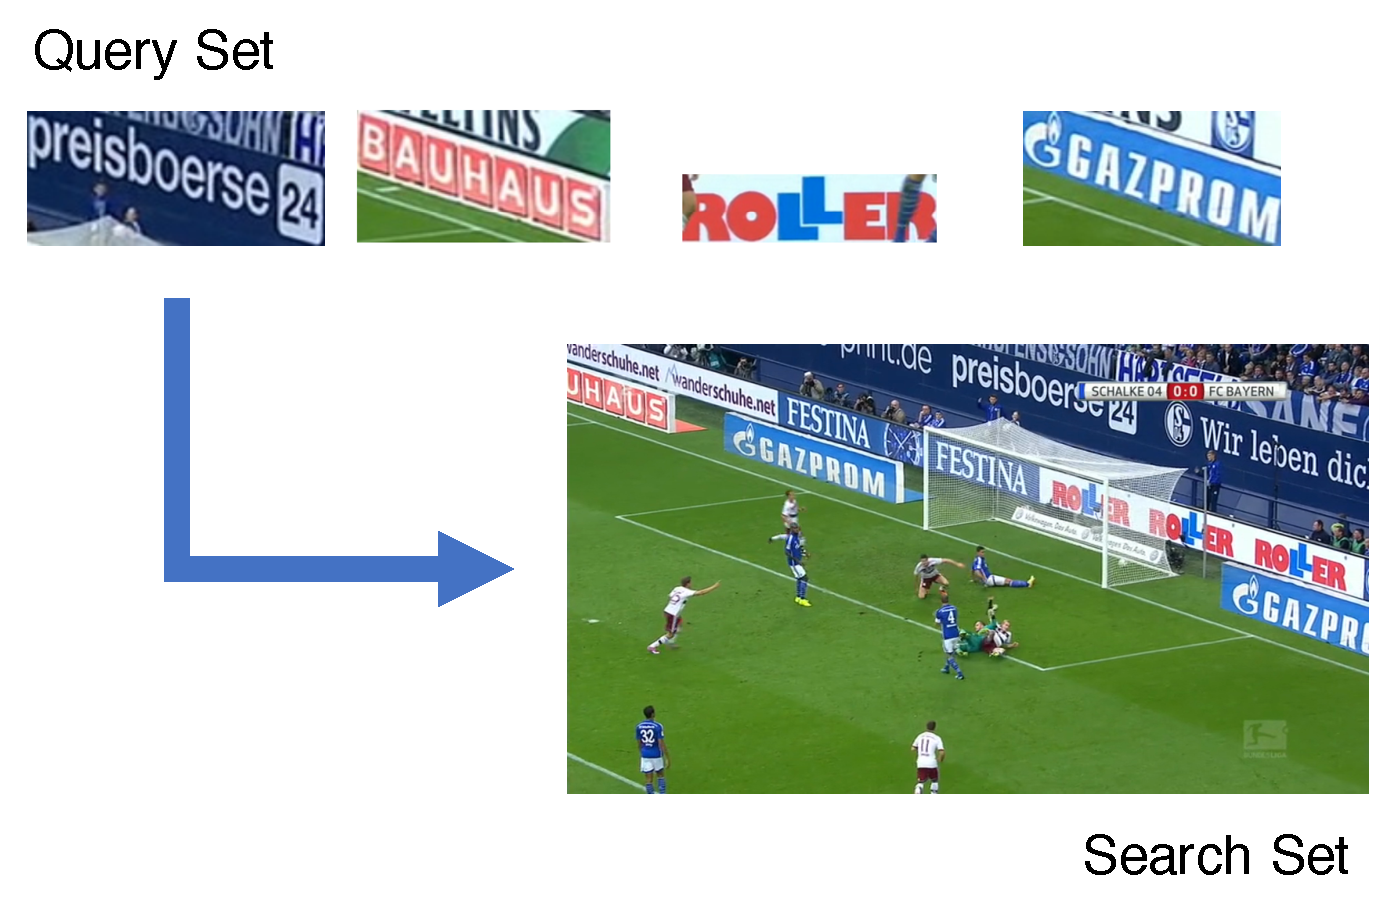
\includegraphics[width=90mm]{querysearch} 
	 \label{f:querysearch}
	\end{figure}
	
\end{frame}

\begin{frame}
	\frametitle{Herausforderungen}
	\bigskip
     	\heading{Logos haben oft schlechte Qualit�t}
   		\begin{figure}
  \centering
  \begin{tabular}{ccccc}
  
\includegraphics[width=15mm]{challenge_1_b.png} &  
\includegraphics[width=15mm]{challenge_2_b.png}  & 
\includegraphics[width=15mm]{challenge_3_b.png} &   
\includegraphics[width=15mm]{challenge_4_b.png} & 
\includegraphics[width=15mm]{challenge_5_b.png} \\
    
\includegraphics[height=10mm]{challenge_1_a.png} &  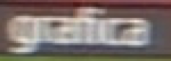
\includegraphics[width=15mm]{challenge_2_a.png}  & 
\includegraphics[width=15mm]{challenge_3_a.png} &  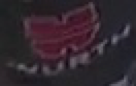
\includegraphics[width=15mm]{challenge_4_a.png}  & 
\includegraphics[width=15mm]{challenge_5_a.png} \\
    \scriptsize{Teilsichtbarkeit} & \scriptsize{Unsch�rfe} & \scriptsize{Perspektivische} & \scriptsize{Ambiente}  & \scriptsize{Aussehenvielfalt} \\
    & & \scriptsize{Transformation}, & \scriptsize{Beleuchtungs�nderung} & \scriptsize{innerhalb} \\
    & & \scriptsize{Rotation} & & \scriptsize{Firmen}
    \end{tabular}
\end{figure}
		 
		 
		  

	\heading{Die Herausforderungen wandeln das Problem in ein Open-Set Wiedererkennungsproblem um}
\end{frame}

\section{Logo Retrieval}

\begin{frame}
	\frametitle{Logo Retrieval}
	\framesubtitle{L�sungsalternativen}
     	\heading{Sliding window method}
	\begin{itemize}
		\item Langsam
		\item Nicht skalierungsinvariant
	\end{itemize}
	\bigskip	
     	\heading{SIFT\textsuperscript{\tiny{0}} oder HOG\textsuperscript{\tiny{1}} Feature Extraktion}
	\begin{itemize}
		\item Seit den letzten Jahren CNNs haben in vielen Problemen bessere Performance
	\end{itemize}
	\bigskip
	\heading{CNN-basierter globaler Deskriptor}
	\begin{itemize}
		\item Von dem ganzen Bild z.B. Szenenwiedererkennung
		\item Ungeeignet f�r kleinere Objekte
	\end{itemize}
	\vfill
	\tiny{[0] Distinctive Image Features from Scale-Invariant Keypoints [Lowe2004]\newline
	[1] Histograms of Oriented Gradients for Human Detection [Dalal2005]}
\end{frame}

\begin{frame}
	\frametitle{Logo Retrieval}
	\framesubtitle{Gew�hlte L�sung}
	\bigskip
	\heading{Proposal-basierte CNNs}
	\begin{itemize}
		     	\item State-of-the-Art L�sung\textsuperscript{\tiny{2}} f�r Closed-Set Logo Retrieval
	\begin{columns}
    		\column{0.25\textwidth}
		\item Fast R-CNN\textsuperscript{\tiny{3}}
		\begin{itemize}
			\item Objektpositionen von externem System
			\item FCN
			\item RoIPolling
		\end{itemize}
		\item Faster R-CNN\textsuperscript{\tiny{4}}
		\begin{itemize}
			\item Objektpositionen von Teilnetz
			\item End-to-End
		\end{itemize}
    		\column{0.2\textwidth}
		\begin{figure}
        			\centering
		        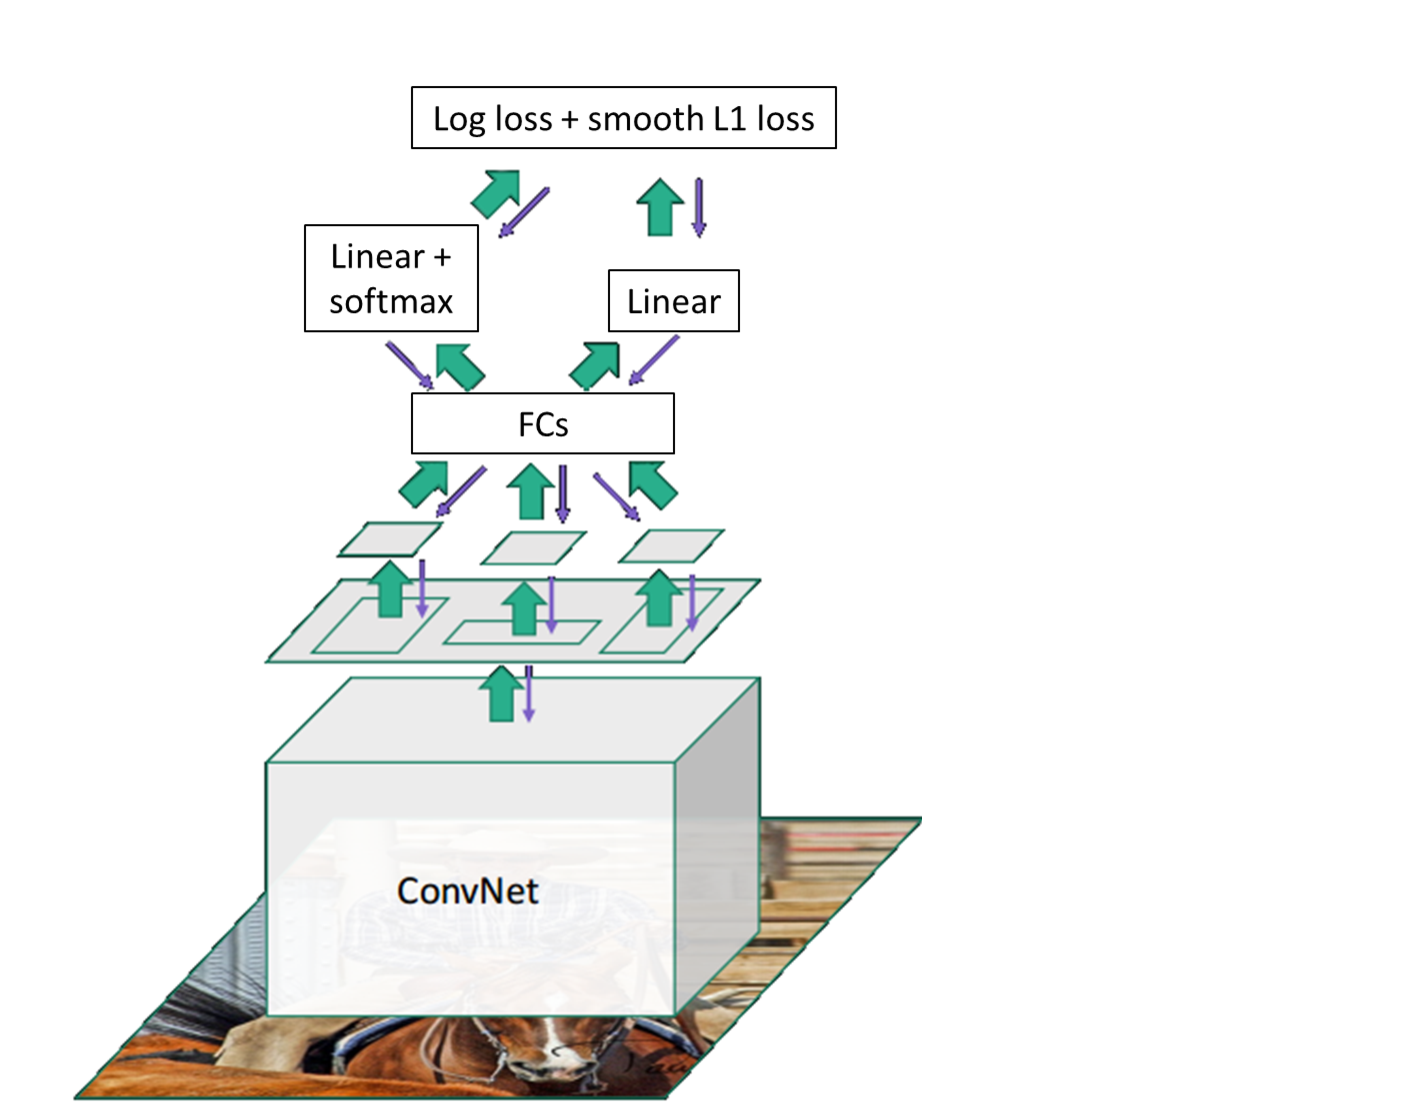
\includegraphics[width=25mm]{fast-rcnn} 
		\end{figure}
		\centering{Fast R-CNN}
    		\column{0.25\textwidth}
		\begin{figure}
        			\centering
		        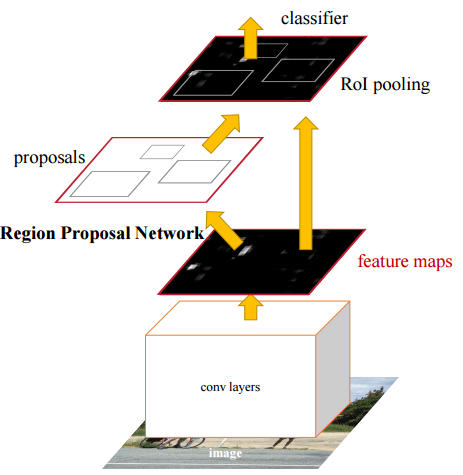
\includegraphics[width=34mm]{faster-rcnn} 
		\end{figure}
		\centering{Faster R-CNN}
	\end{columns}
	\end{itemize}
	\vfill
	\tiny{[2] Fast R-CNN [Girshick2015]\newline
	[3] Faster R-CNN: Towards Real-Time Object Detection with Region Proposal Networks [Girshick2015]\newline
	[4] Region-based CNN for Logo Detection [Bao2016]}
\end{frame}

\section{Das vorgestellte Logo Retrieval System}

\begin{frame}
	\frametitle{Logo Retrieval System}
	\bigskip
	\heading{Das Problem ist anders}
	\begin{itemize}
		\item Open-Set, weil verschiedene Logos im Training-Set als im Test-Set
	\end{itemize}		
     	\heading{Die L�sung ist in zwei Teile aufgeteilt}
	\begin{itemize}
		\item Logo Detektion
		\begin{itemize}
			\item Um alle Arten von Logo-Bilder zu erkennen
			\item Funktioniert ohne Anfragebilder
		\end{itemize}
		\item Logo Vergleich
		\begin{itemize}
			\item Die Feature Vektoren von Regionen werden extrahiert
			\item Vergleich miteinander
		\end{itemize}
	\end{itemize}
	\begin{figure}
        \centering
        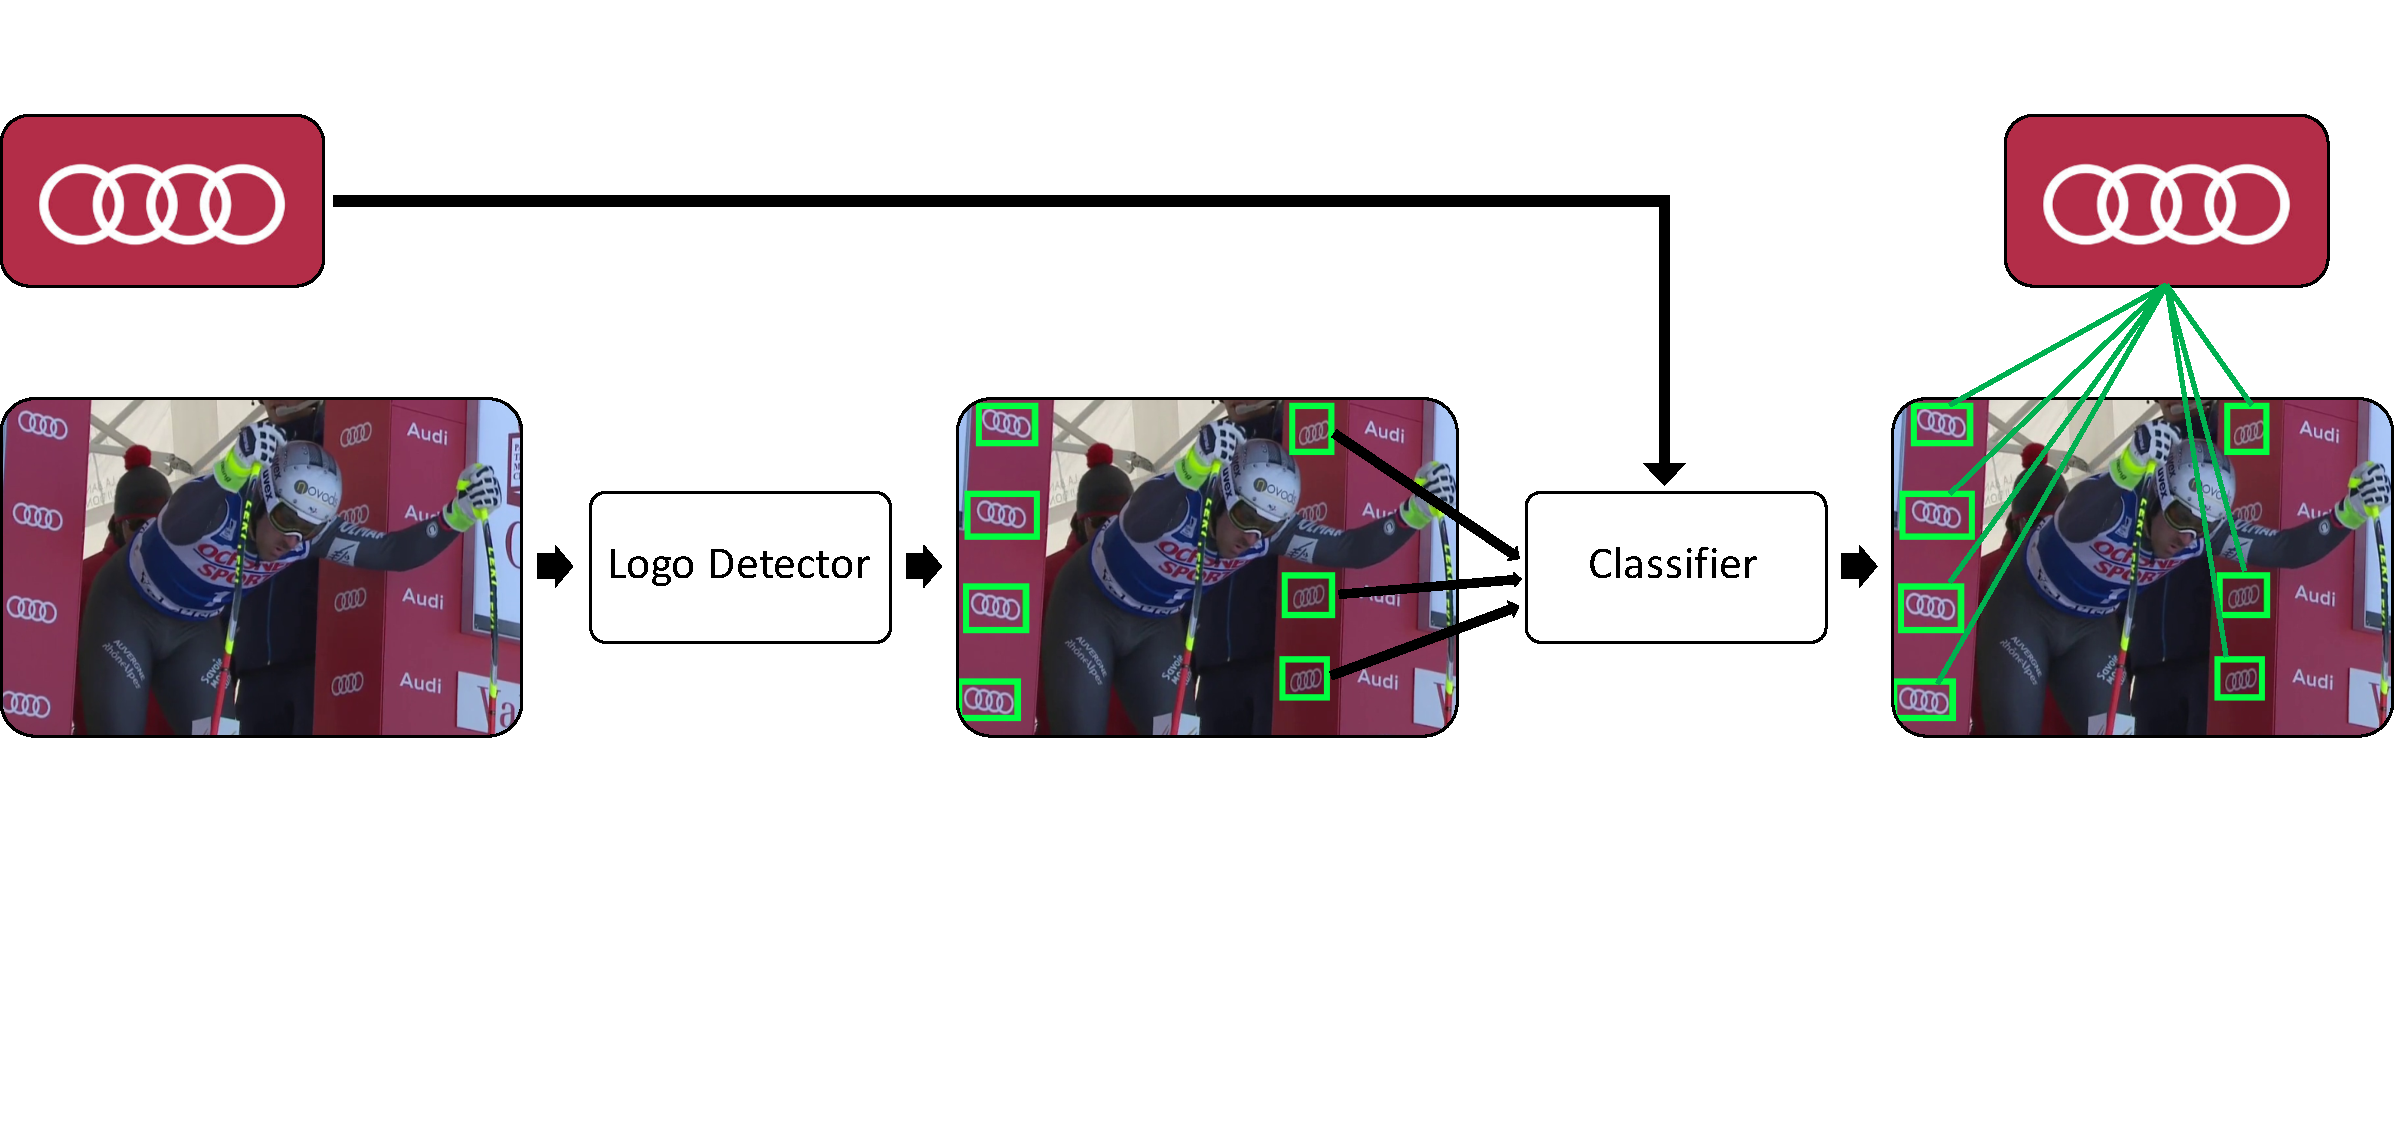
\includegraphics[width=110mm]{outline} 
	 \label{f:outline}
	\end{figure}
\end{frame}

\begin{frame}
	\frametitle{Logo Retrieval System}
	\heading{Logo Detektion}
	\begin{itemize}
		\item Neun Architekturen trainiert und evaluiert
		\item Effekt von unterschiedliche Training-Datens�tze untersucht
		\item Zwei Typen ausgew�hlt und vorgestellt
	\end{itemize}
	\begin{figure}
        		\centering
	        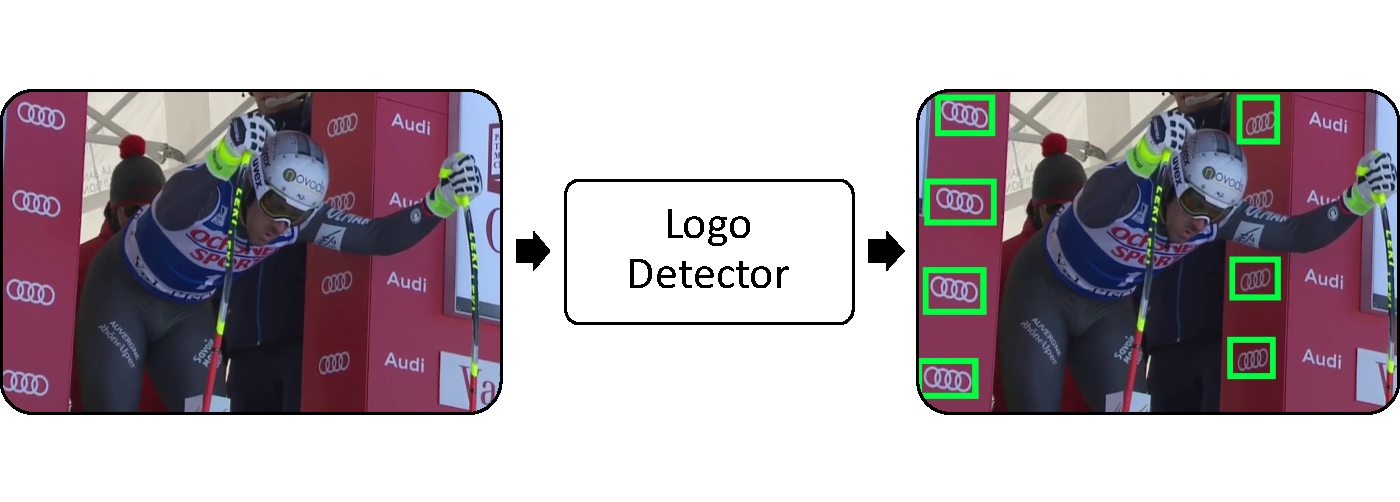
\includegraphics[width=100mm]{logodetection} 
	\end{figure}
\end{frame}

\begin{frame}
	\frametitle{Logo Retrieval System}
	\framesubtitle{Logo Detektion}
	\begin{columns}
    		\column{0.6\textwidth}
		\heading{Region Proposal Network Logo Detektor}
		\begin{itemize}
			\item Wird gleichzeitig mit dem Faster R-CNN Netz trainiert
			\item Extrahierbar aus einem schon trainierten Netz
			\item Sucht auf der Feature Map in Sliding-Window-Fashion
			\item Vordefinierte Anzahl von Anchor-Boxen
			\begin{itemize}
				\item Offset wird trainiert, angewendet auf den Anchor-Boxen
			\end{itemize}
		\end{itemize}
	    	\column{0.4\textwidth}
		\begin{figure}
		        \centering
		        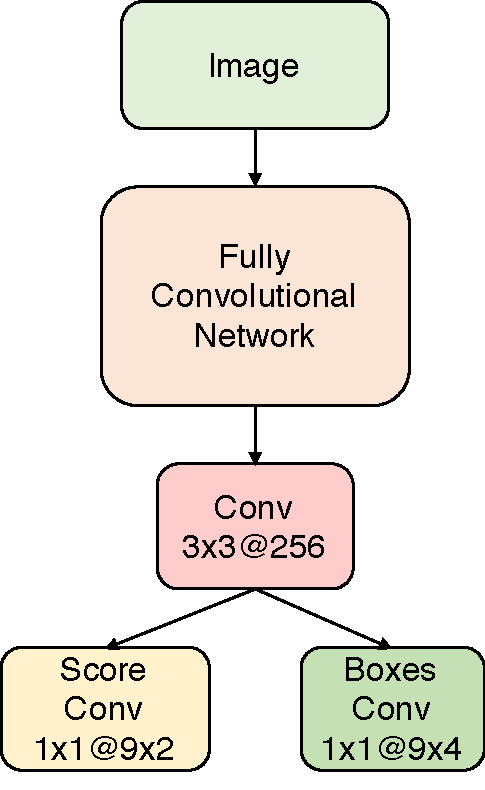
\includegraphics[height=60mm]{rpndetektion} 
		        \label{f:rpndetektion}
		\end{figure}
	\end{columns}
\end{frame}

\begin{frame}
	\frametitle{Logo Retrieval System}
	\framesubtitle{Logo Detektion}
	\begin{columns}
    		\column{0.6\textwidth}
		\heading{Faster R-CNN Logo Detektor}
		\begin{itemize}
			\item Trainiert f�r zwei Klassen
			\item RPN Teil kann als schwacher Klassifikator betrachtet werden
			\item Zusammen ergeben eine Kaskade von Detektoren
		\end{itemize}
    		\column{0.4\textwidth}
		\begin{figure}
	        \centering
        		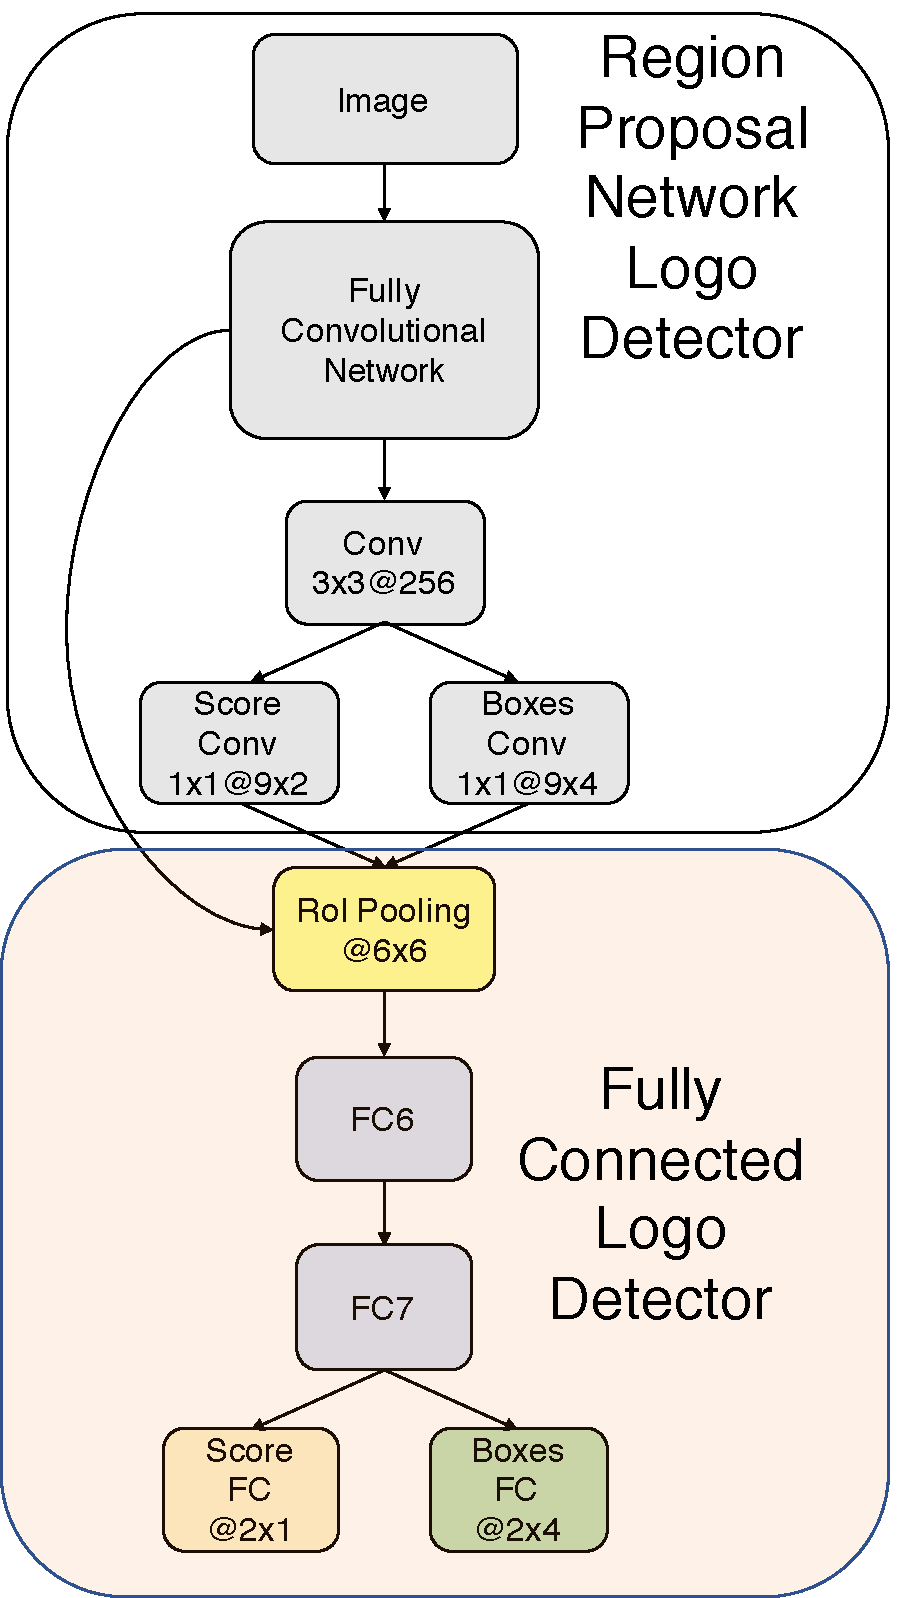
\includegraphics[height=70mm]{classagnosticdetektion} 
		 \label{f:classagnosticdetektion}
		\end{figure}
	\end{columns}
\end{frame}

\begin{frame}
	\frametitle{Logo Retrieval System}
	\heading{Logo Vergleich}
	\begin{itemize}
		\item Zw�lf verschiedene Archtitekturen trainiert und evaluiert
		\item Effekt von unterschiedliche Training-Datens�tze untersucht
		\item Vier Typen ausgew�hlt und vorgestellt
	\end{itemize}
	\begin{figure}
        		\centering
	        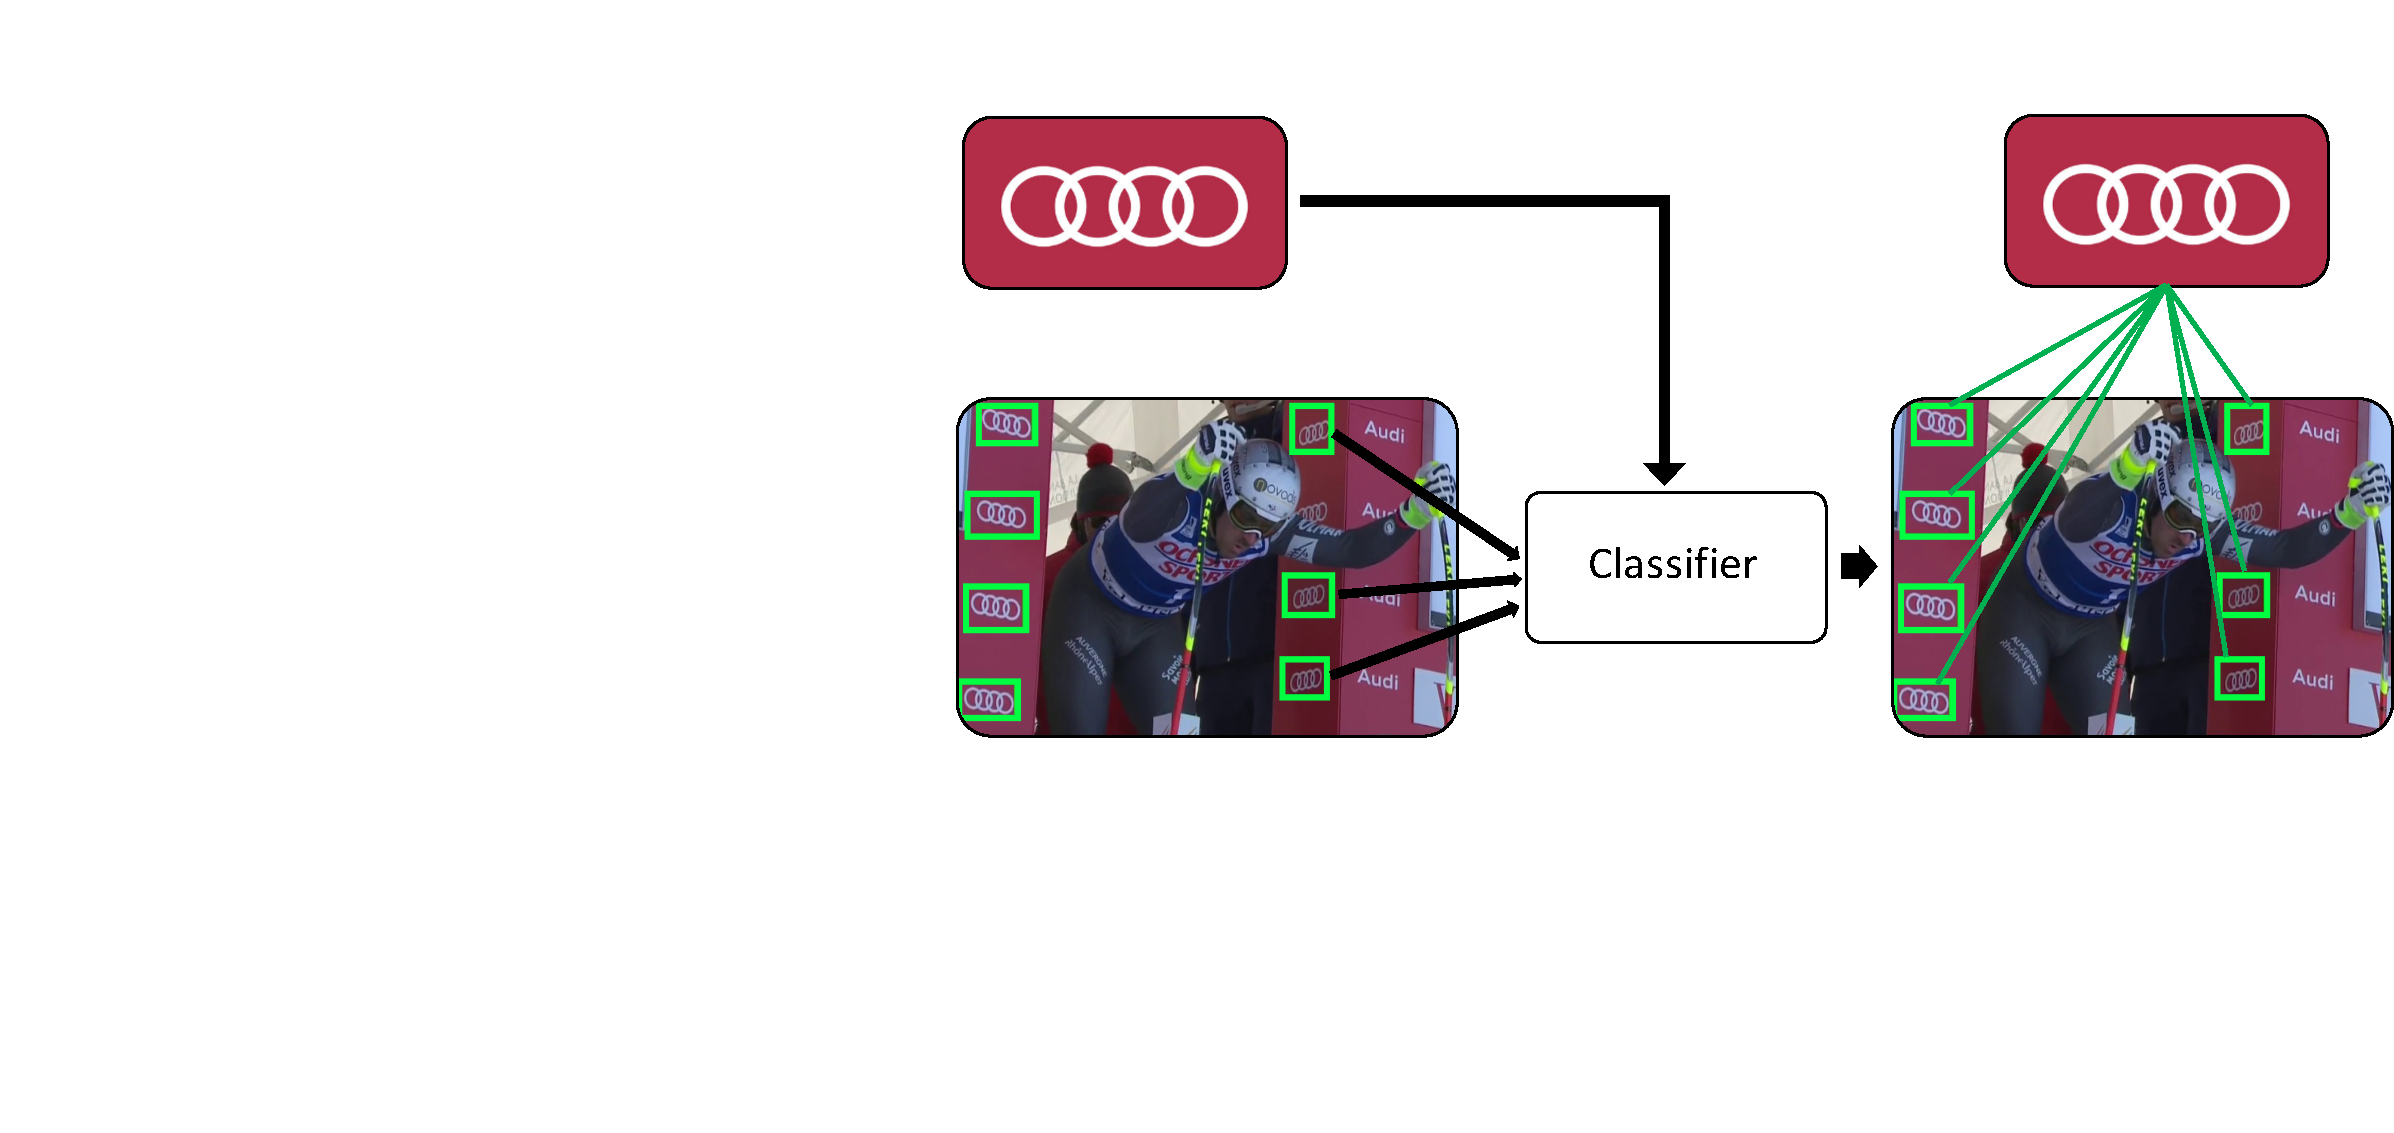
\includegraphics[width=100mm]{logocomparison} 
	\end{figure}
\end{frame}

\begin{frame}
	\frametitle{Logo Retrieval System}
	\framesubtitle{Logo Vergleich}
	\begin{columns}
    		\column{0.47\textwidth}
		\heading{Faster-Logos - Baseline}
		\begin{itemize}
			\item State-of-the-Art in Closed-Set Logo Retrieval
			\item Grundlage: Faster R-CNN
			\item Angepasst f�r Open-Set
			\item Die Score Ausgabe von RPN wird f�r Detektion benutzt
			\item Klassenwahrscheinlichkeiten werden als Features benutzt
			\item F�r Anfragebild, die Bounding-Box mit der h�chsten Detektionsscore
		\end{itemize}
    		\column{0.53\textwidth}
		\begin{figure}
	        \centering
        		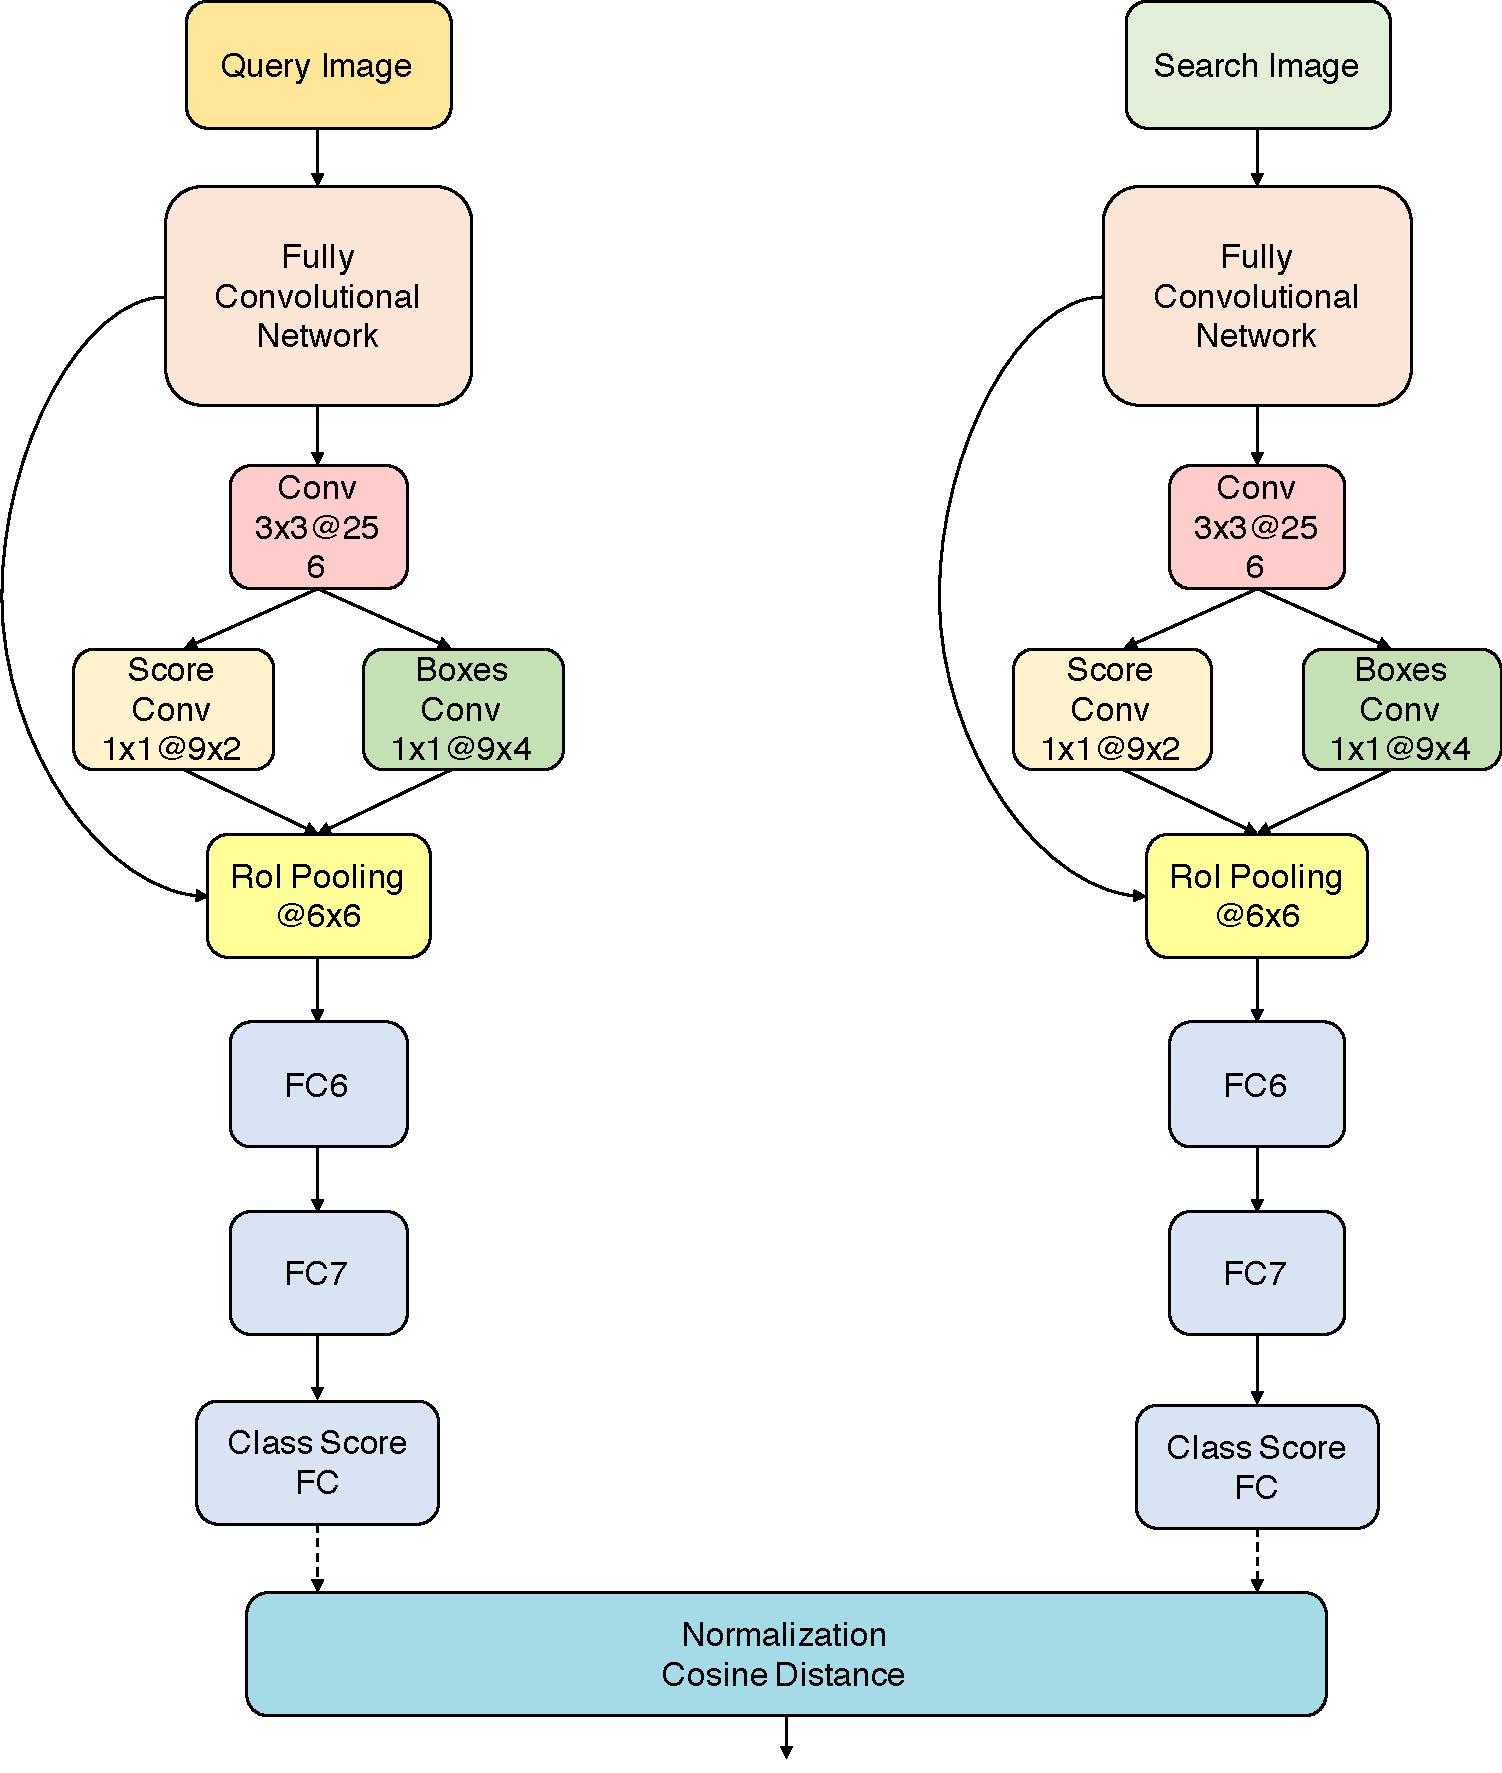
\includegraphics[height=65mm]{sol1_arch} 
		\end{figure}
	\end{columns}
\end{frame}

\begin{frame}
	\frametitle{Logo Retrieval System}
	\framesubtitle{Logo Vergleich}
	\begin{columns}
    		\column{0.47\textwidth}
		\heading{Komplettanfragebild}
		\begin{itemize}
			\item Oft falsche Bounding-Box-Vorhersage von Anfragebild
			\item Entspricht f�r Fast R-CNN
			\item Nachteil: die Logos sollen gut zugeschnitten werden
		\end{itemize}
		\begin{figure}
	        \centering
        		
\includegraphics[height=20mm]{missdet} 
		\end{figure}
    		\column{0.53\textwidth}
		\begin{figure}
	        \centering
        		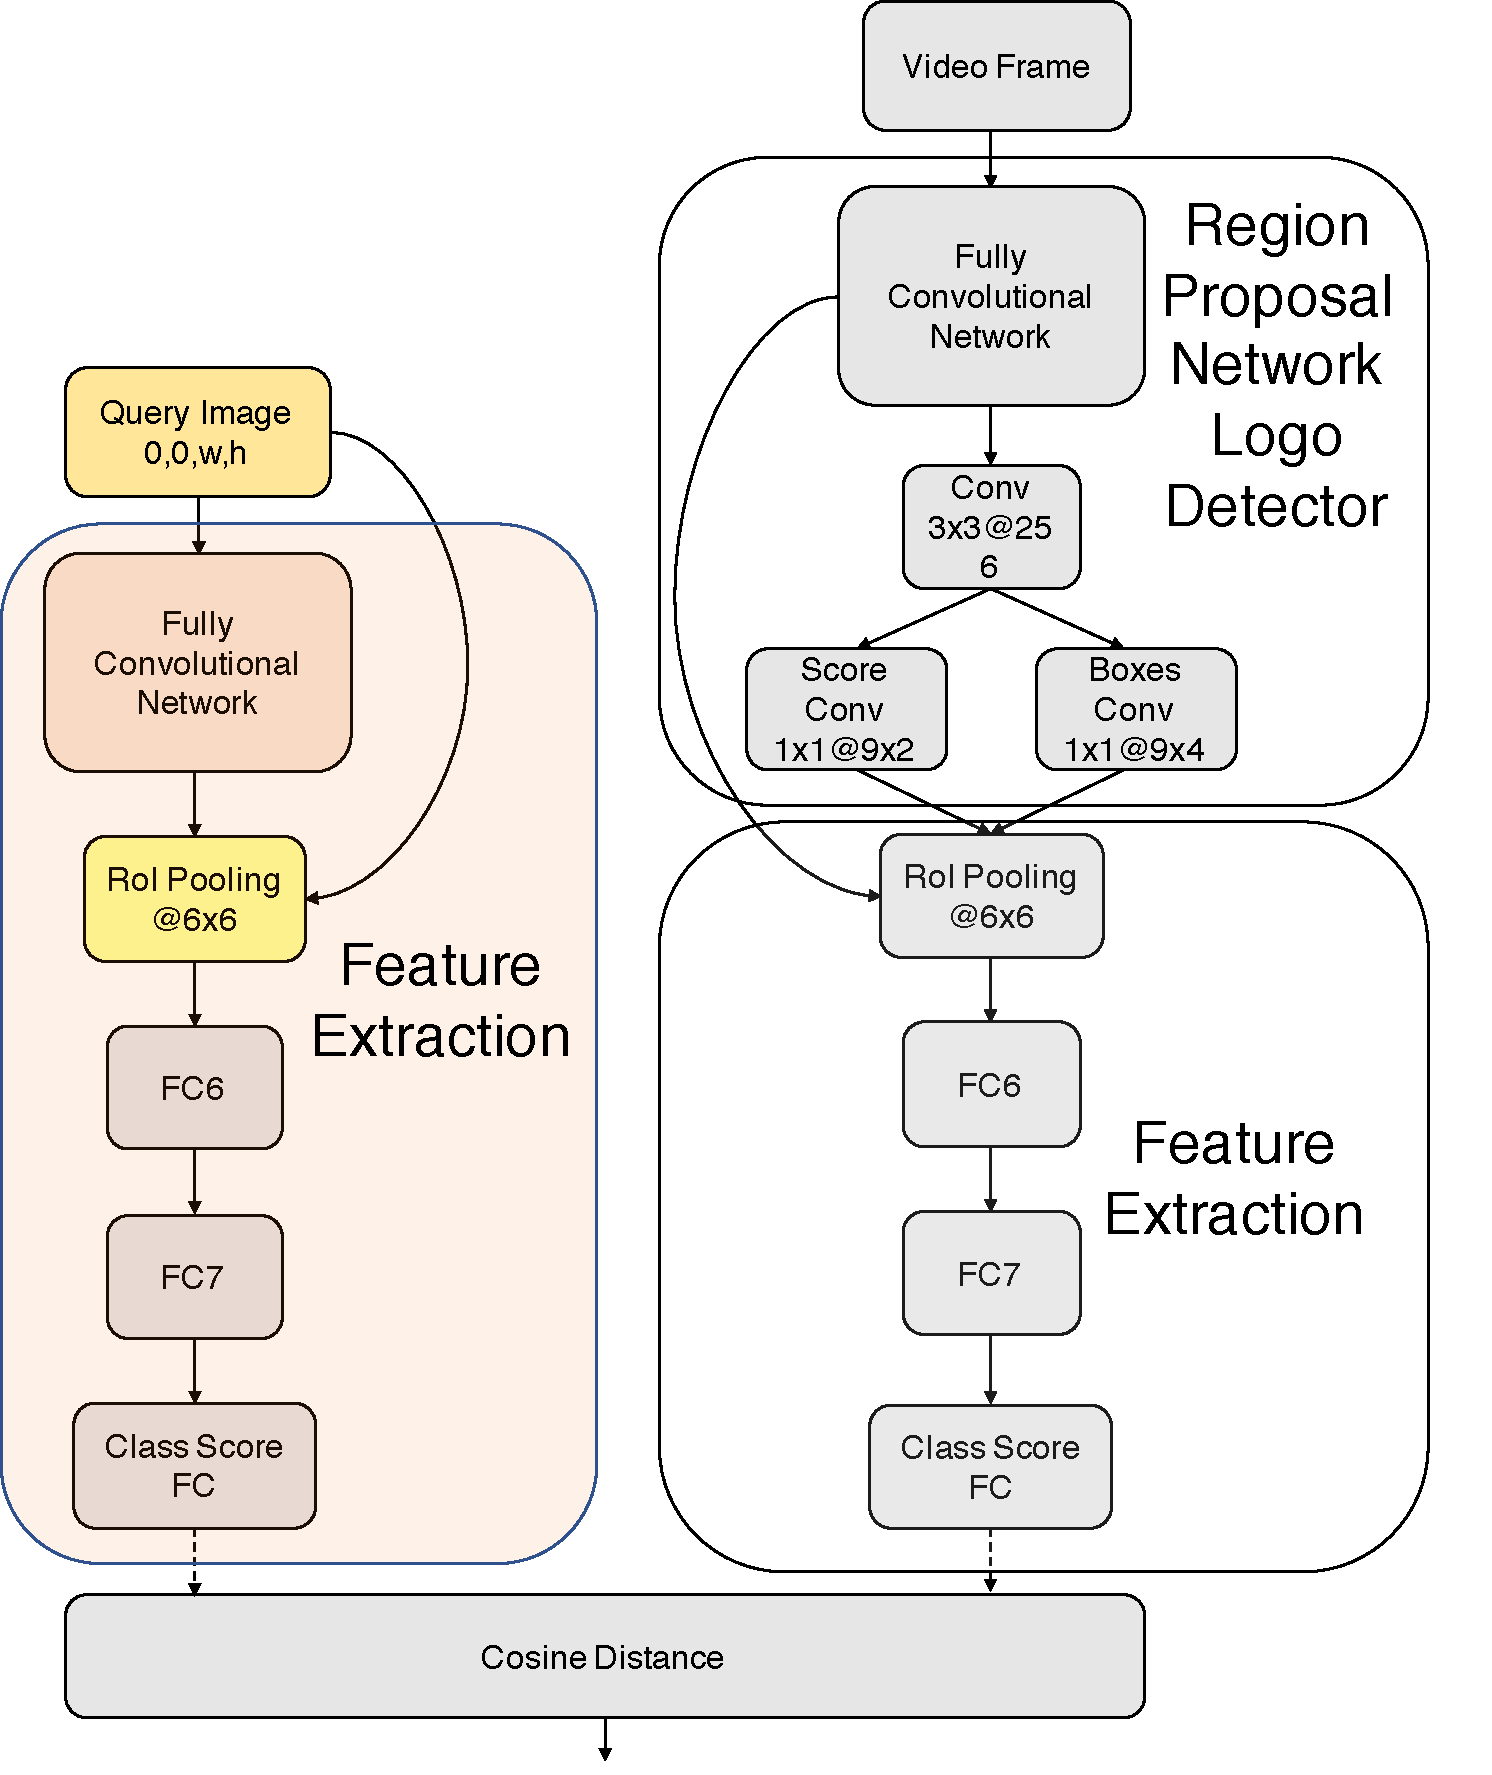
\includegraphics[height=70mm]{sol2_arch} 
		\end{figure}
	\end{columns}
\end{frame}

\begin{frame}
	\frametitle{Logo Retrieval System}
	\framesubtitle{Logo Vergleich}
	\bigskip
	\begin{columns}
    		\column{0.47\textwidth}
		\heading{Siam-Logos}
		\begin{itemize}
			\item Siamesisches Netz\textsuperscript{\tiny{6}}, trainiert gemeinsam sowohl f�r Detektion als auch f�r Klassifikation
			\item Gewichte von FCN und RPN sind geteilt zwischen die �ste des Netzes
			\item Die Ausgabe des Detektors ist f�r Objektness Score benutzt
			\item Das Netz kann weitertrainiert werden, wenn es noch zus�tzliche Logo-Daten ohne spezifisches Brand-Label gibt
		\end{itemize}
    		\column{0.53\textwidth}
		\begin{figure}
	        \centering
        		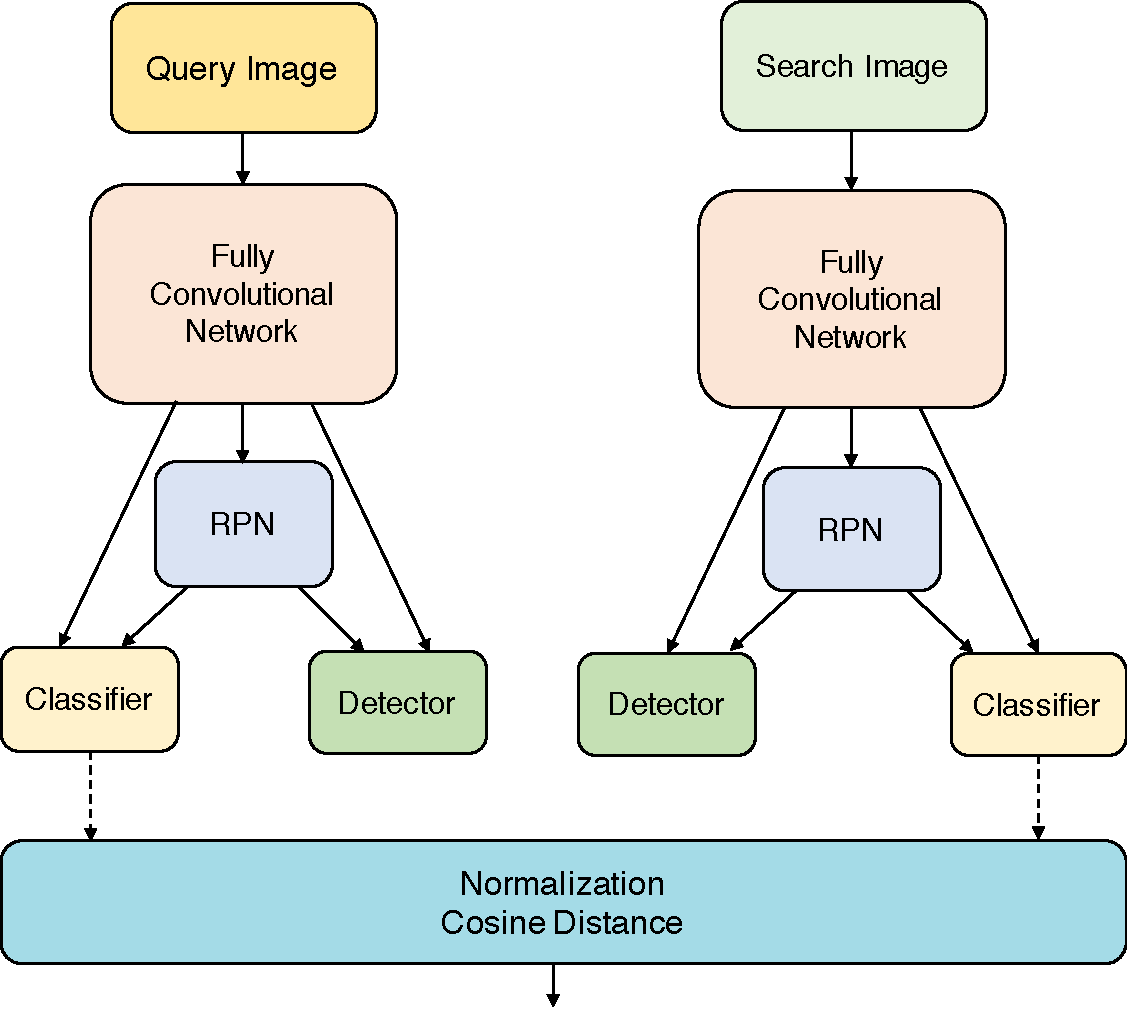
\includegraphics[height=40mm]{sol5_arch_test} 
		\end{figure}
		\centering{Test Phase}
	\end{columns}
	\vfill
	\tiny{[6] Signature verification using a \textquote{Siamese} time delay neural network [Bromley1993]}
\end{frame}


\begin{frame}
	\frametitle{Logo Retrieval System}
	\framesubtitle{Logo Vergleich}
	\bigskip
	\heading{Separater Detektor und Klassifikator}
	\begin{columns}
    		\column{0.4\textwidth}
		\begin{itemize}
			\item Probleme
			\begin{itemize}
				\item Merkmale von Feature Map zwischen Detektion und Merkmalsextraktion geteilt
				\item Keine Spezialisation auf die eigentliche Aufgabe
			\end{itemize}
			\item Idee: Trennung von Detektor und Klassifikator
			\item Vorteile
			\begin{itemize}
				\item Alle state-of-the-art Netze verwendbar f�r Feature Extraktion
				\item Flexibler in Bezug auf vortrainierten Netze als mit Fast-Faster R-CNN
			\end{itemize}
		\end{itemize}
    		\column{0.5\textwidth}
		\begin{figure}
	        \centering
        		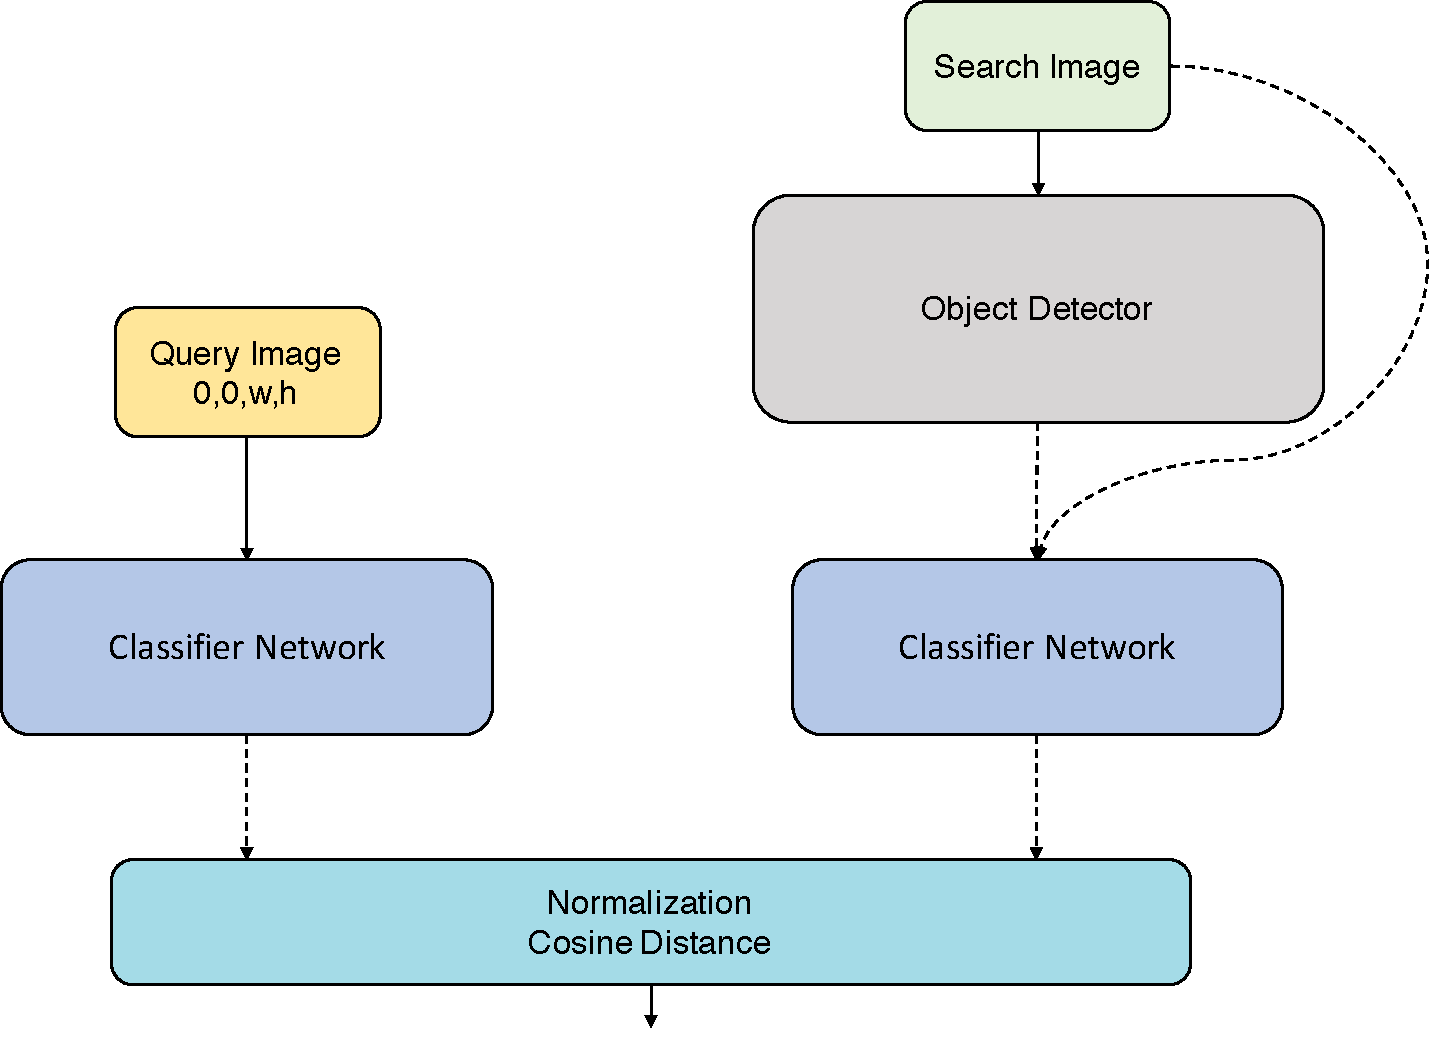
\includegraphics[height=40mm]{sol4_arch} 
		\end{figure}
	\end{columns}
\end{frame}

\section{Logo Datens�tze}

\begin{frame}
	\frametitle{Logo Datens�tze}
	\begin{columns}
    		\column{0.45\textwidth}
		\bigskip
		\heading{�ffentliche Datens�tze}
		\begin{itemize}
			\item BelgaLogos-32\textsuperscript{\tiny{7}}, FlickrBelgaLogos\textsuperscript{\tiny{8}}, Flickr Logos 27\textsuperscript{\tiny{9}}, FlickrLogos-32\textsuperscript{\tiny{10}}, Logos-32Plus\textsuperscript{\tiny{11}}, TopLogo-10\textsuperscript{\tiny{12}}
		\end{itemize}
		\heading{Selbst-annotierte Datens�tze - SportLogos}
		\begin{itemize}
			\item Football-1, Football-2, Ski, IceHockey
		\end{itemize}
    		\column{0.55\textwidth}
		\begin{figure}
	        \centering
        		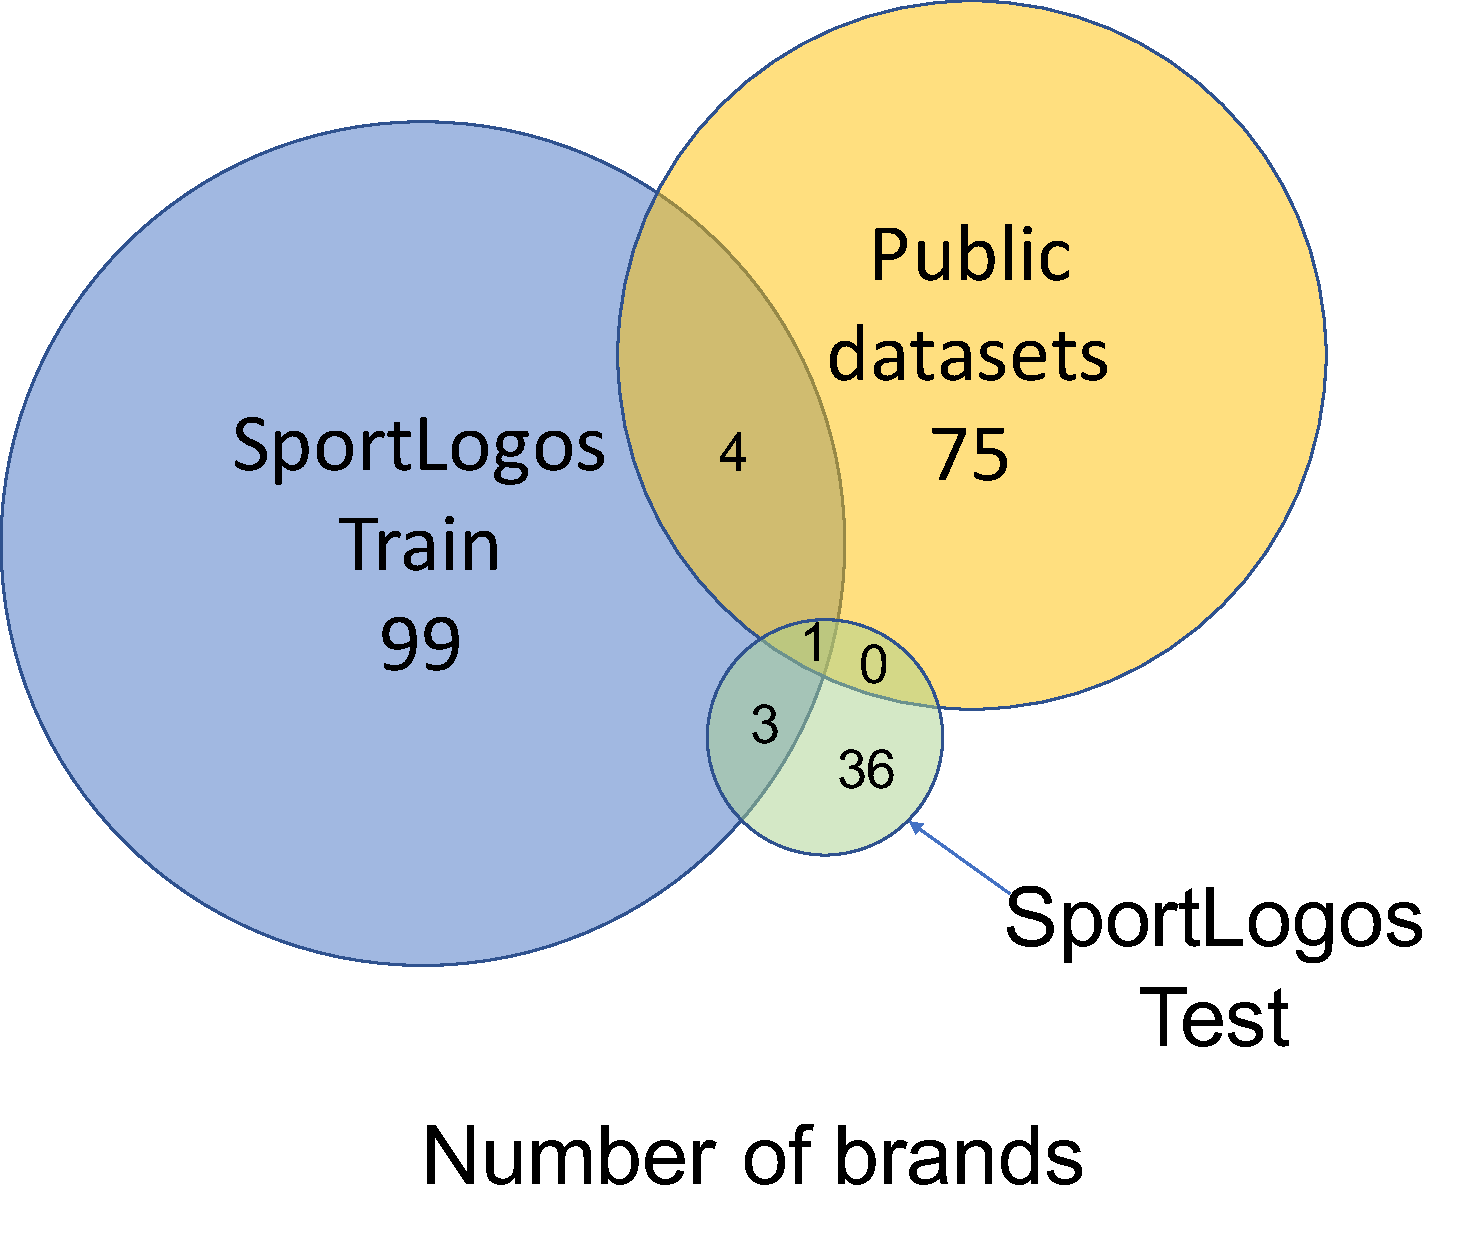
\includegraphics[height=40mm]{brandintersections} 
		\end{figure}
	\end{columns}
	\begin{figure}
	        \centering
        		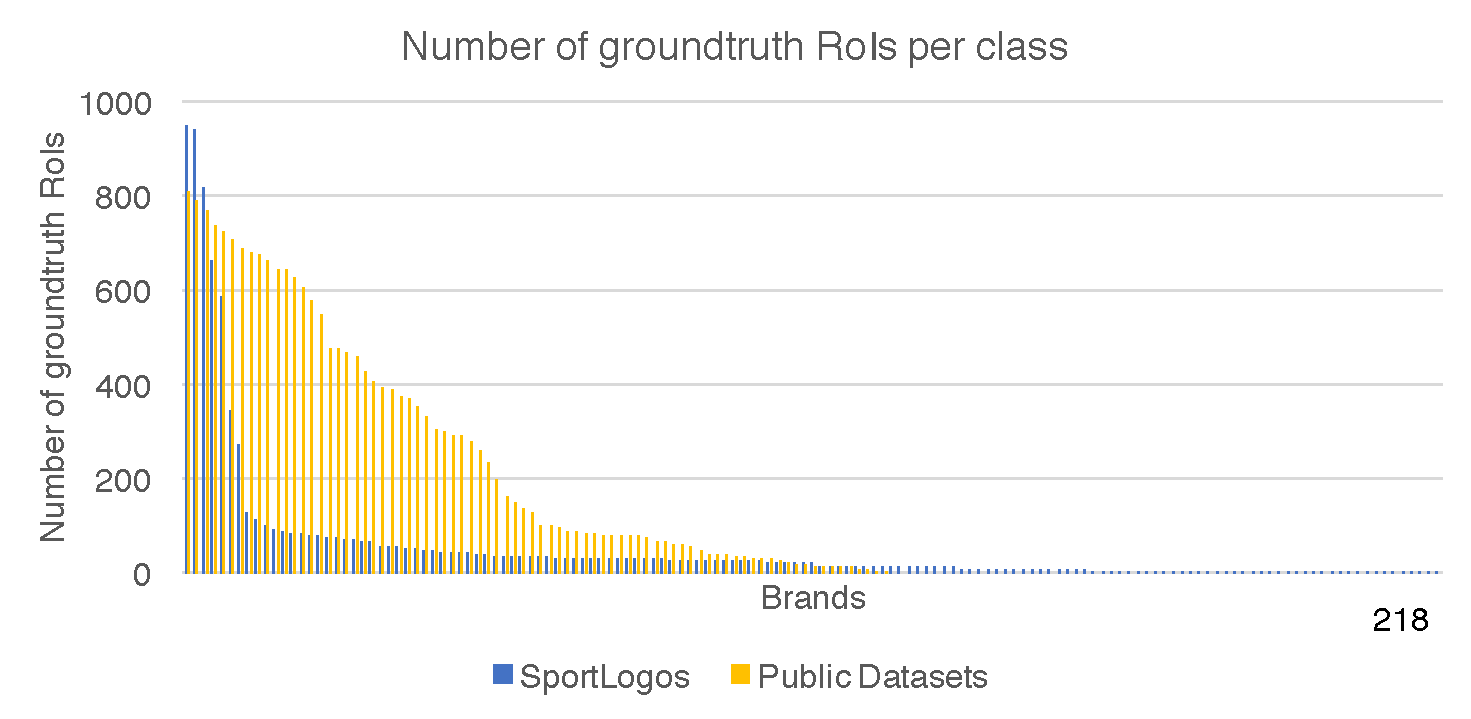
\includegraphics[height=35mm]{branddistribution} 
	\end{figure}
\end{frame}

\begin{frame}
	\frametitle{Logo Datens�tze}
	\bigskip
	\begin{tabular}{ccccc}
		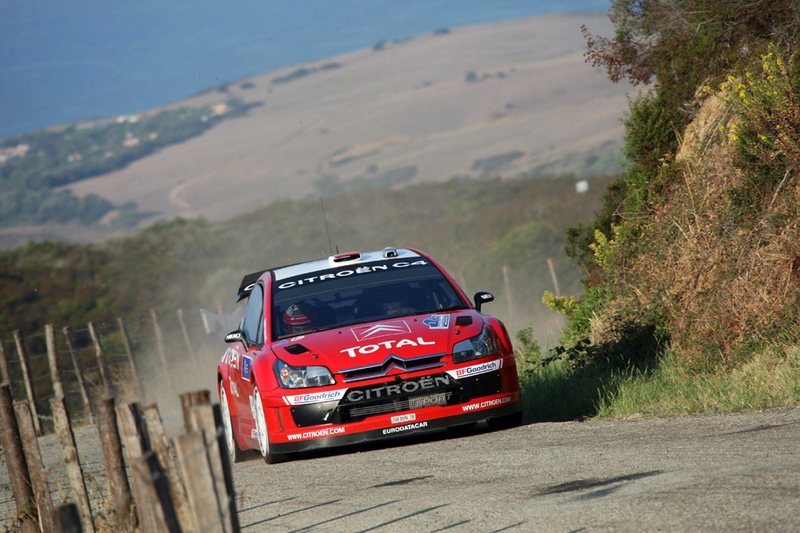
\includegraphics[width=29mm]{belga} & &  \includegraphics[width=29mm]{Flickrlogos27}  & & 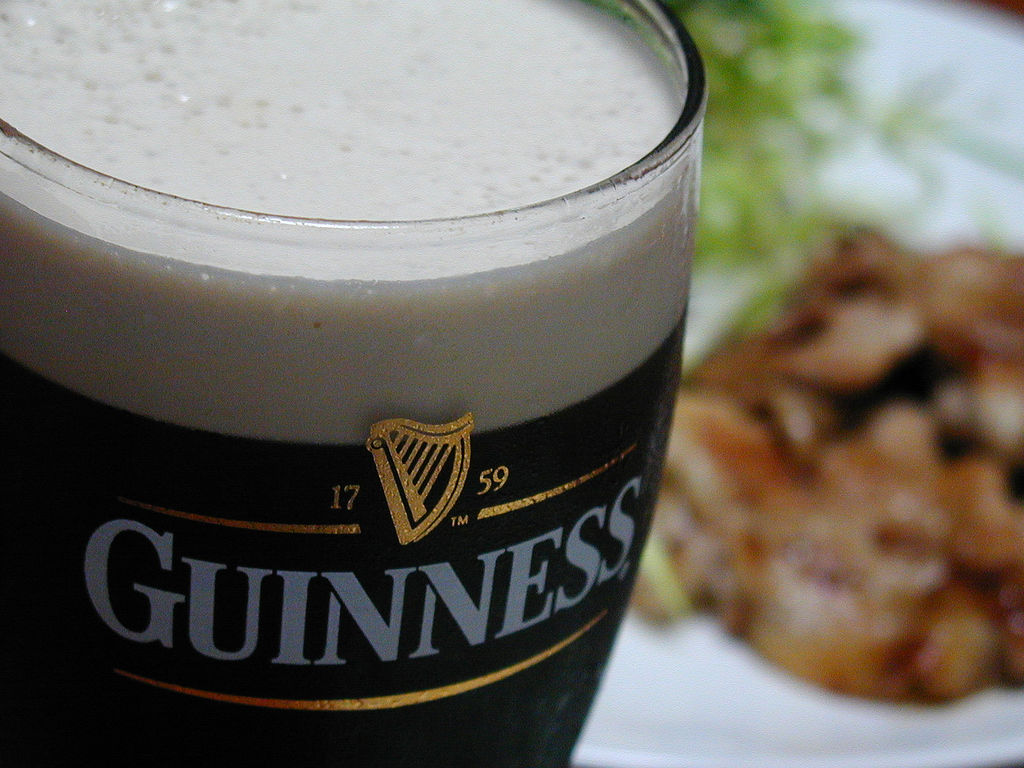
\includegraphics[width=29mm]{flickr32} \\
		BelgaLogos & & Flickr Logos 27 & & FlickrLogos-32 \\
		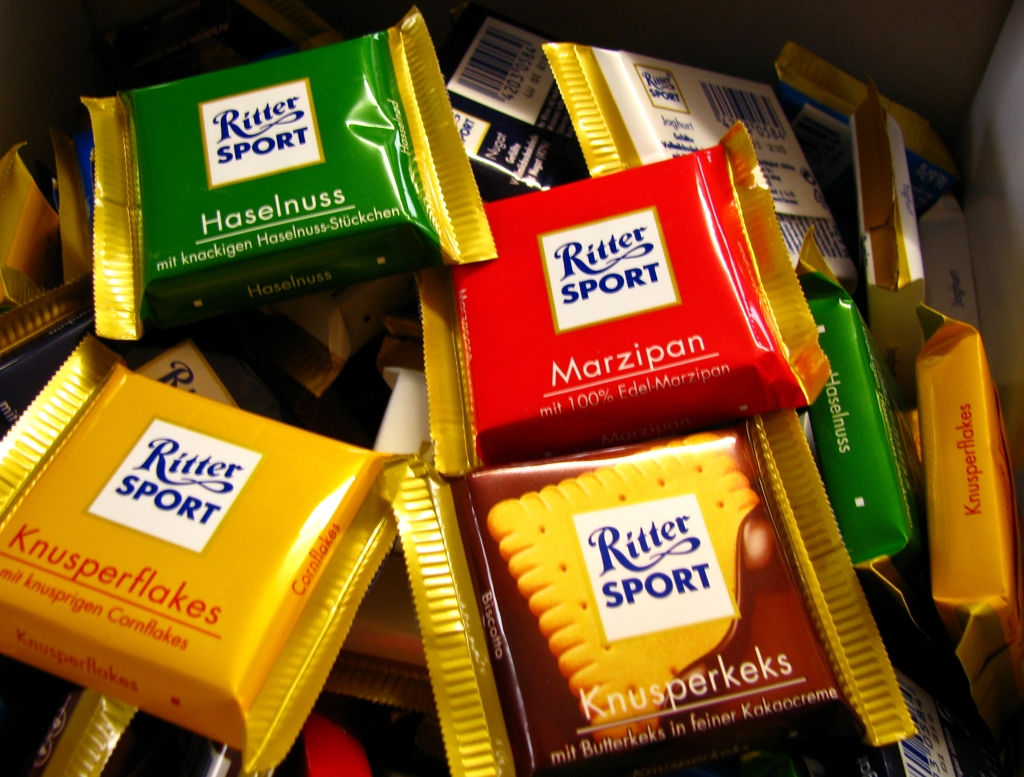
\includegraphics[width=29mm]{logos32plus} & &  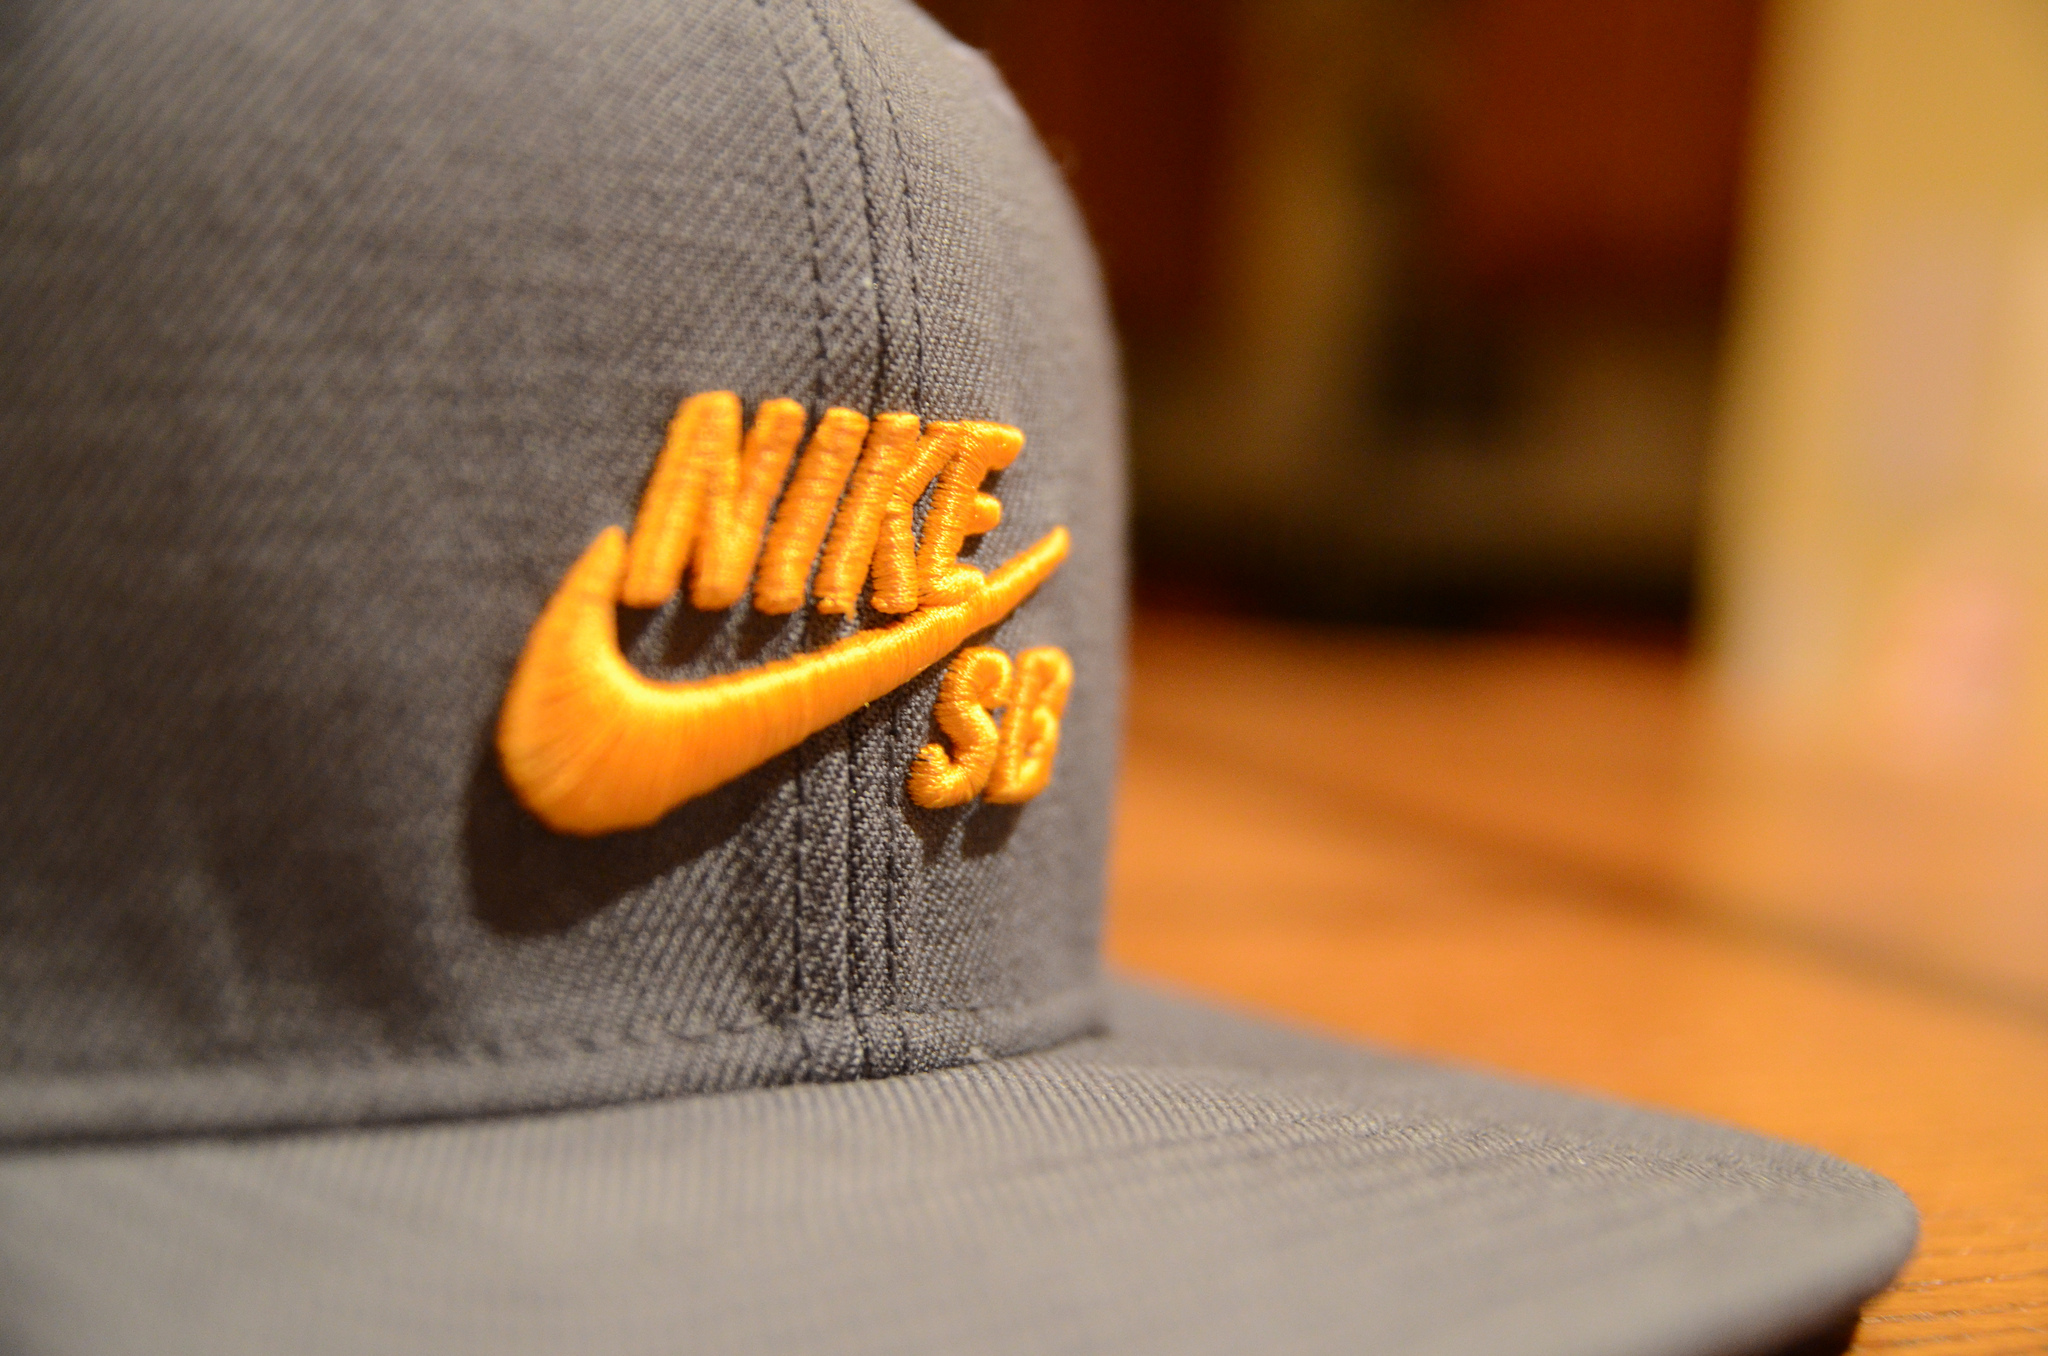
\includegraphics[width=29mm]{toplogo10}  & & 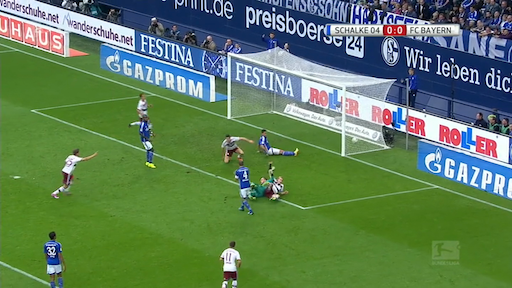
\includegraphics[width=29mm]{sportlogos} \\
		Logos-32Plus & & TopLogo-10 & & SportLogos
	\end{tabular}
\end{frame}

\section{Evaluation}

\begin{frame}
	\frametitle{Evaluation}
	\heading{Verwendeter Test Set}
	\begin{itemize}
		\item SportLogos: Football-2
	\end{itemize}
	\bigskip
	\heading{Anfragebilder}
	\begin{itemize}
		\item Von dem Video ausgeschnitten
	\end{itemize}
	\heading{Detection Rate}
	\begin{itemize}
		\item Dargestellt �ber die Durchschnittsanzahl von falschen Detektionen
		\item Gleich mit Recall, True Positive Rate
	\end{itemize}
	\heading{Detection Identification Rate}
	\begin{itemize}
		\item Gibt einen holistischen �berblick �ber die Leistung des gesamten Retrieval-Systems
		\item Als Funktion der Durchschnittsanzahl von falschen Klassifikationen
	\end{itemize}
\end{frame}

\begin{frame}
\frametitle{Evaluation}
	\heading{Logo Detektion Vergleich}
	\begin{figure}
	        \centering
       		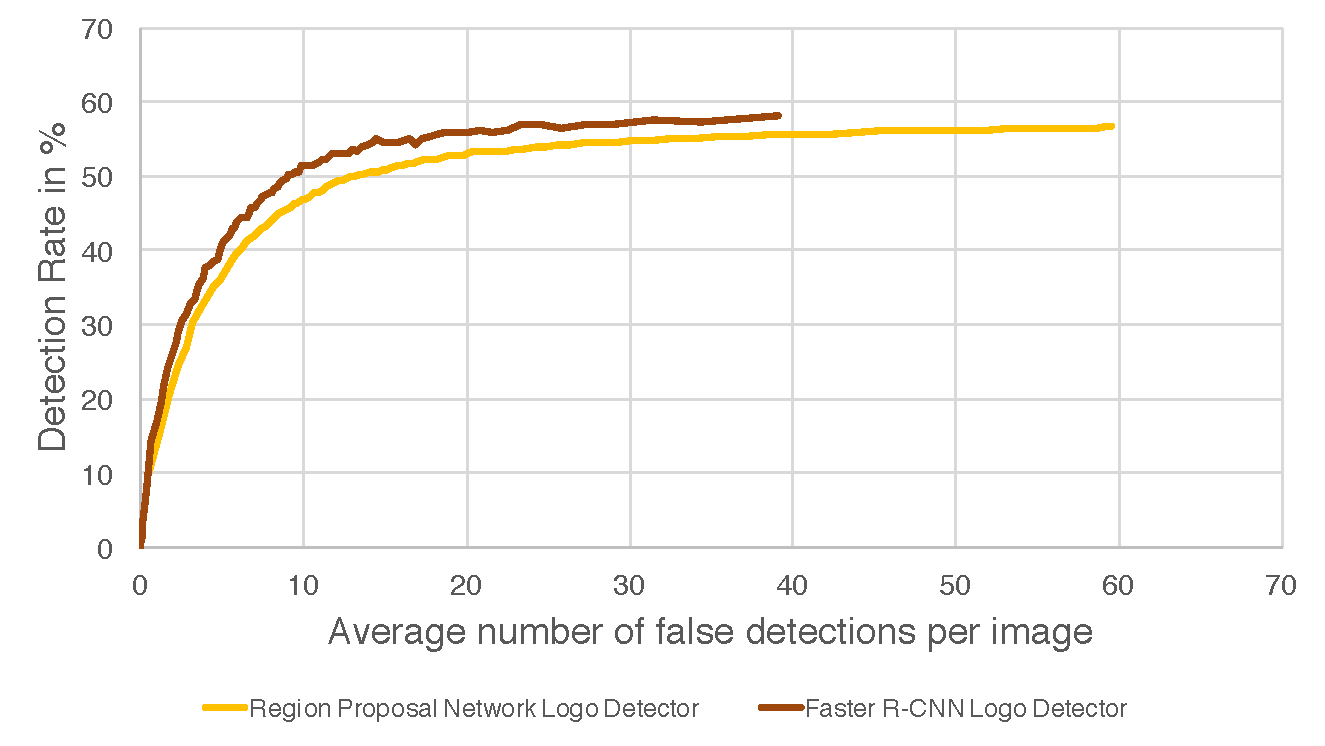
\includegraphics[height=55mm]{deteval} 
	\end{figure}
\end{frame}

\begin{frame}
\frametitle{Evaluation}
	\heading{Logo Detektion Beispiel}
\includemedia[width=108mm,height=60mm,activate=pageopen,
passcontext,
transparent,
addresource=test_full.mp4,
flashvars={source=test_full.mp4}
]{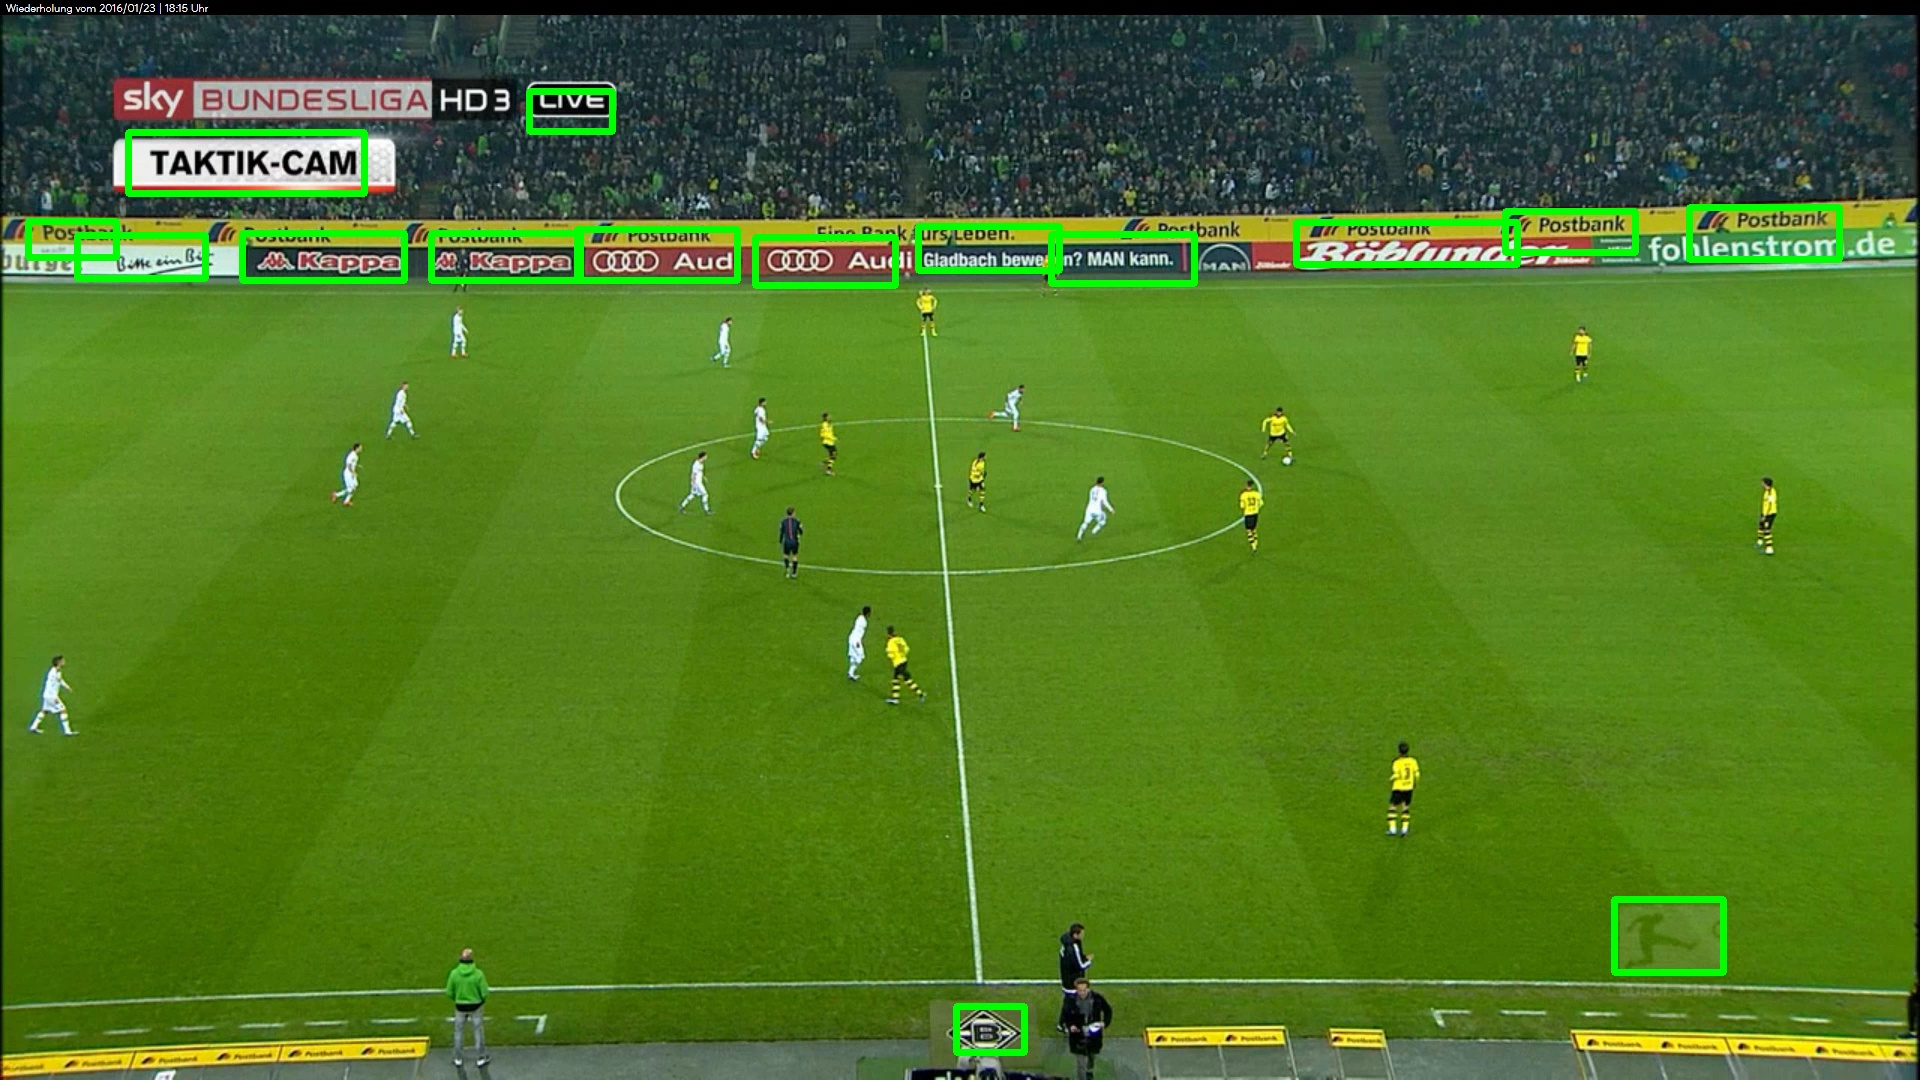
\includegraphics[width=108mm]{vidframe.jpg}}{VPlayer.swf}

  \end{frame}

\begin{frame}
	\frametitle{Evaluation}
	\heading{Logo Retrieval Vergleich}
	\begin{figure}
	        \centering
       		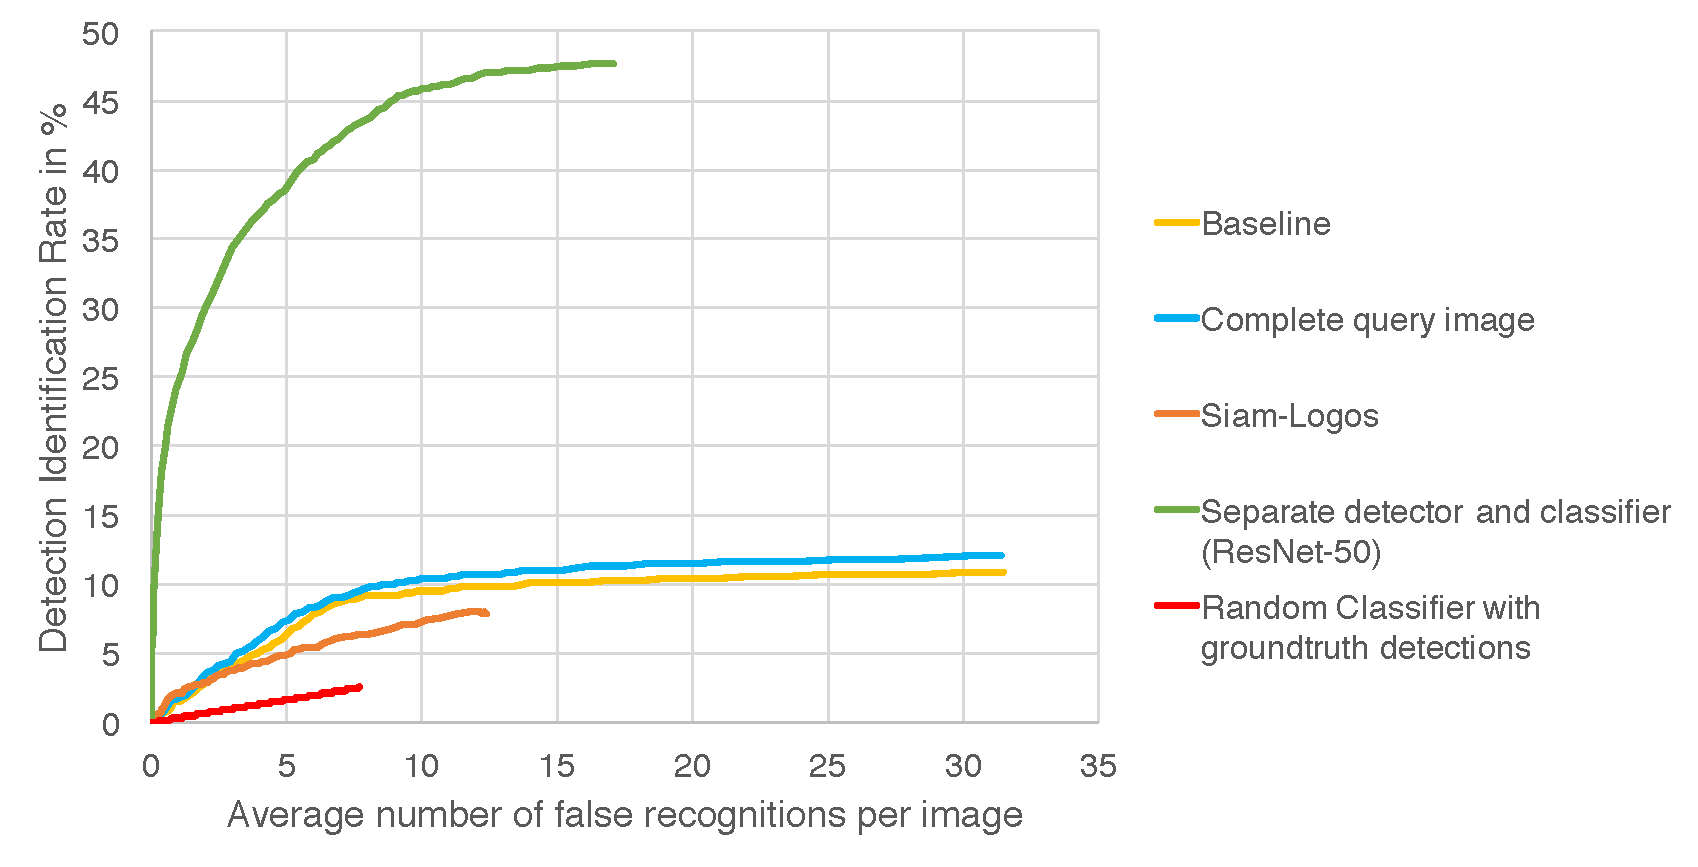
\includegraphics[height=55mm]{clseval} 
	\end{figure}
\end{frame}

\begin{frame}
	\frametitle{Evaluation}
	\heading{Logo Retrieval Beispiel}
	\begin{figure}
	        \centering
       		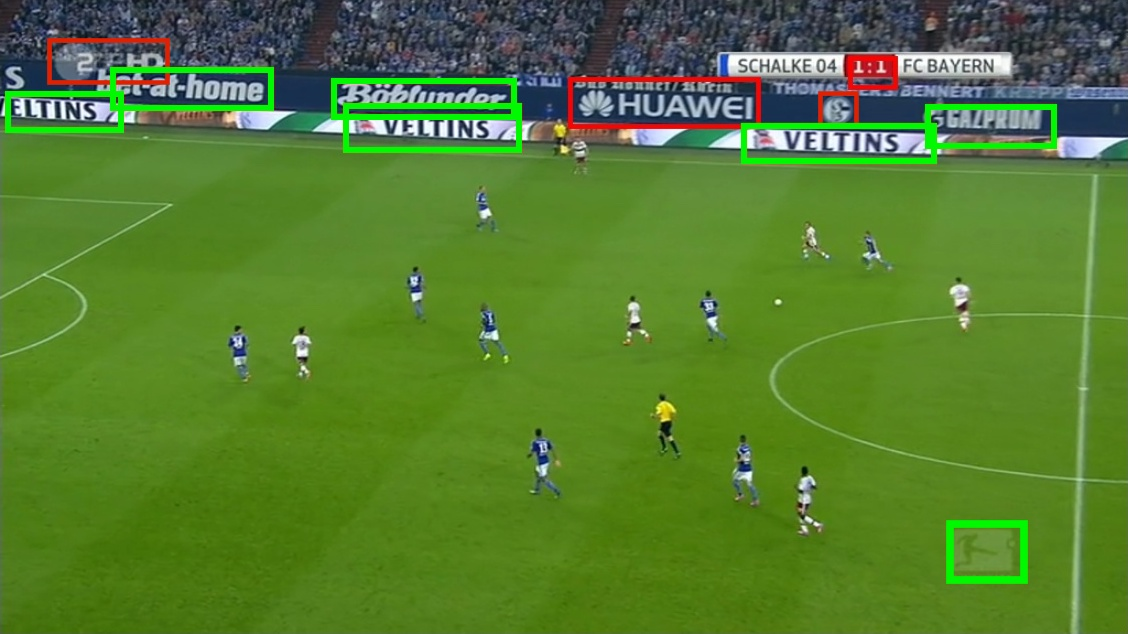
\includegraphics[height=55mm]{cls} 
	\end{figure}
\end{frame}

\section{Zusammenfassung und Ausblick}

\begin{frame}
	\frametitle{Zusammenfassung und Ausblick}
	\begin{columns}
    		\column{0.5\textwidth}
		\heading{Zusammenfassung}
		\begin{itemize}
			\item Logo System vorgestellt f�r Open Set Retrieval
			\item Erreicht 47\% auf dem Test Datensatz
			\item Schwierigkeiten
			\begin{itemize}
				\item Schlechte Qualit�t
				\item Aussehenvielfalt
			\end{itemize}
		\end{itemize}
    		\column{0.4\textwidth}
		\begin{figure}
	        		\centering
	       		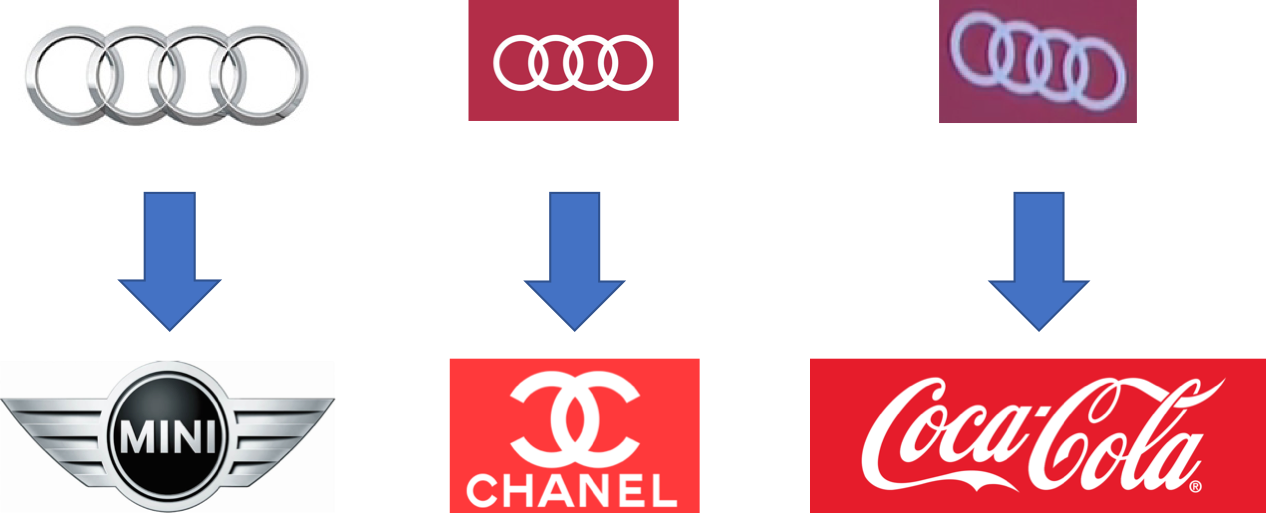
\includegraphics[height=25mm]{confusion} 
		\end{figure}
	\end{columns}
	\heading{Ausblick}
	\begin{itemize}
		\item Textbasierte Logos
		\begin{itemize}
			\item �berwiegende Mehrheit der Logos ist textbasiert
			\item Erweiterung des Systems mit Texterkennung-Subsystem
		\end{itemize}

		\item Logo Tracking
		\begin{itemize}
			\item Erg�nzung bei fehlender Detektion 
			\item Reduzierung einmaliger Fehlklassifikation der getrackten Objekte
		\end{itemize}
		\item Mehr Daten
		\begin{itemize}
			\item Die Gr��e der fusionierten Logo Datens�tzen ist zu klein f�r Deep Learning
		\end{itemize}
	\end{itemize}
\end{frame}
%-------------------------------------------------------
\transl{%
\section*{End}}{%
\section*{Ende}}
%-------------------------------------------------------

%-------------------------------------------------------
%  The end
%-------------------------------------------------------
\begin{frame}
	\frametitle{\hyperlink{Outline}{\transl{%
			The End}{%
			Ende}}}
	\centering
		\hyperlink{Backup-Outline}{
\includegraphics[width=3cm]{questionmark}}
%	\pause
\end{frame}

% intro
\section{}

\begin{frame}
	\frametitle{Weitere Bibliografie}
	[7] Logo retrieval with a contrario visual query expansion [Alexis2009]\newline
	[8] Scalable mining of small visual objects [Alexis2012]\newline
	[9] Scalable Triangulation-based Logo Recognition [Kalantidis2011]\newline
	[10] Scalable logo recognition in real-world images [Romberg2011]\newline
	[11] Deep learning for logo recognition [Bianco2017]\newline
	[12] Deep Learning Logo Detection with Data Expansion by Synthesising Context [Su2016]
\end{frame}

\begin{frame}
	\center\Huge Anhang
\end{frame}

\begin{frame}
	\frametitle{Siam-Logos Test Phase}
	\begin{figure}
	        \centering
        		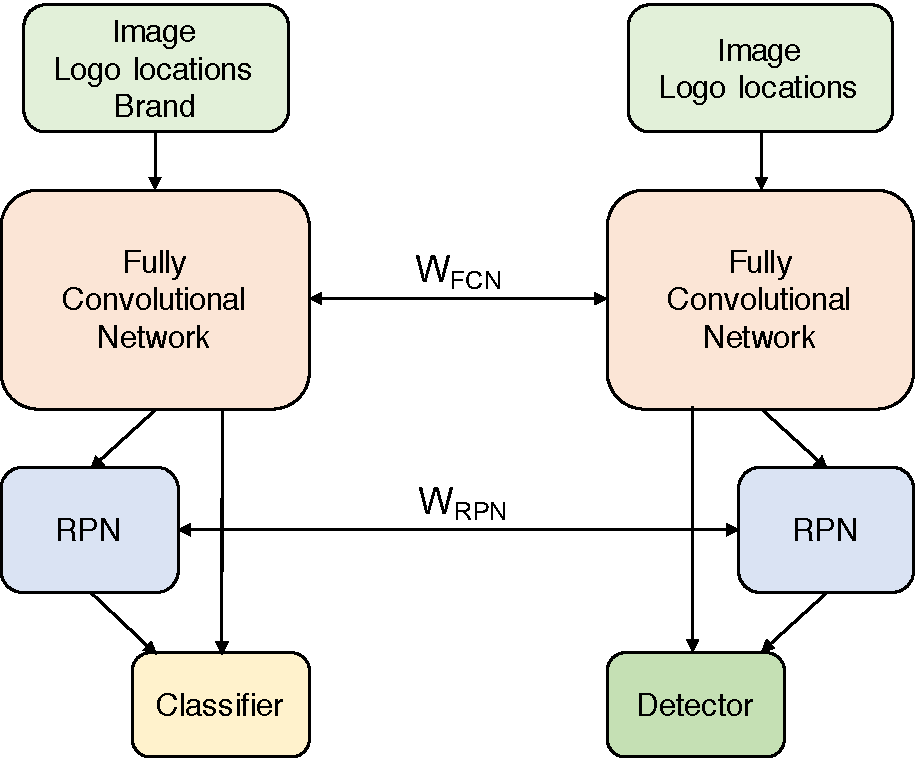
\includegraphics[height=60mm]{sol5_arch_train} 
	\end{figure}
\end{frame}

\begin{frame}
	\frametitle{�hnlichkeitsscores}
	\begin{figure}
	        \centering
        		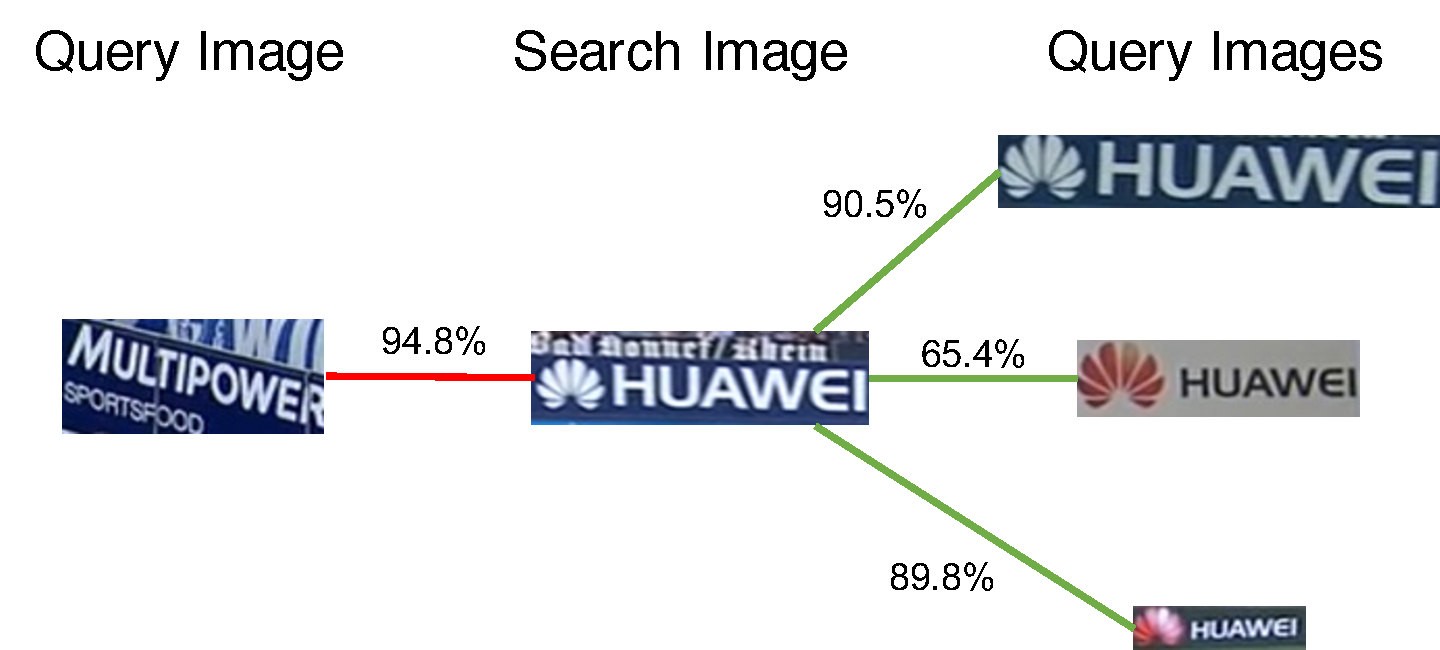
\includegraphics[height=50mm]{cosdistance} 
	\end{figure}
\end{frame}

\begin{frame}
\frametitle{Evaluation}
	\heading{Logo Detektion}
	\begin{figure}
	        \centering
       		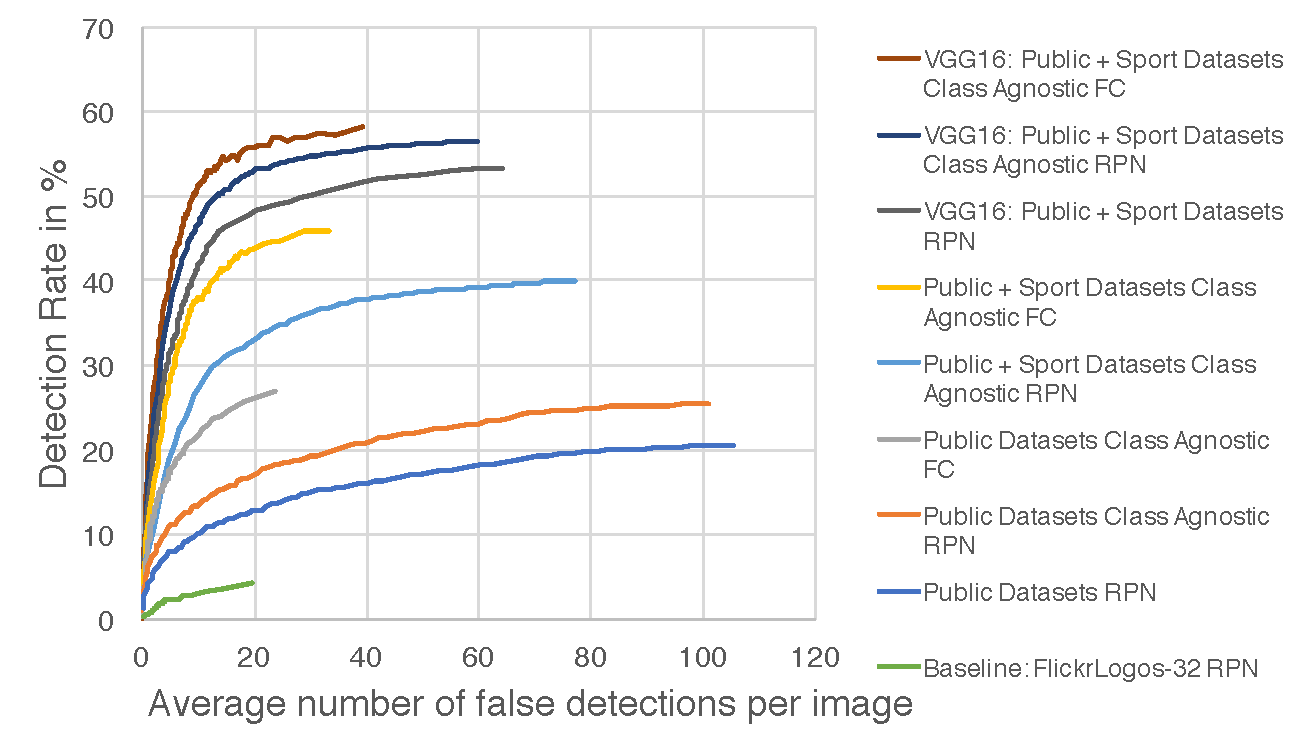
\includegraphics[height=55mm]{detection_full} 
	\end{figure}
\end{frame}

\begin{frame}
	\frametitle{Evaluation}
	\heading{Fast-Logos, Fast	\&Faster-Logos vs. Baseline}
	\begin{figure}
	        \centering
       		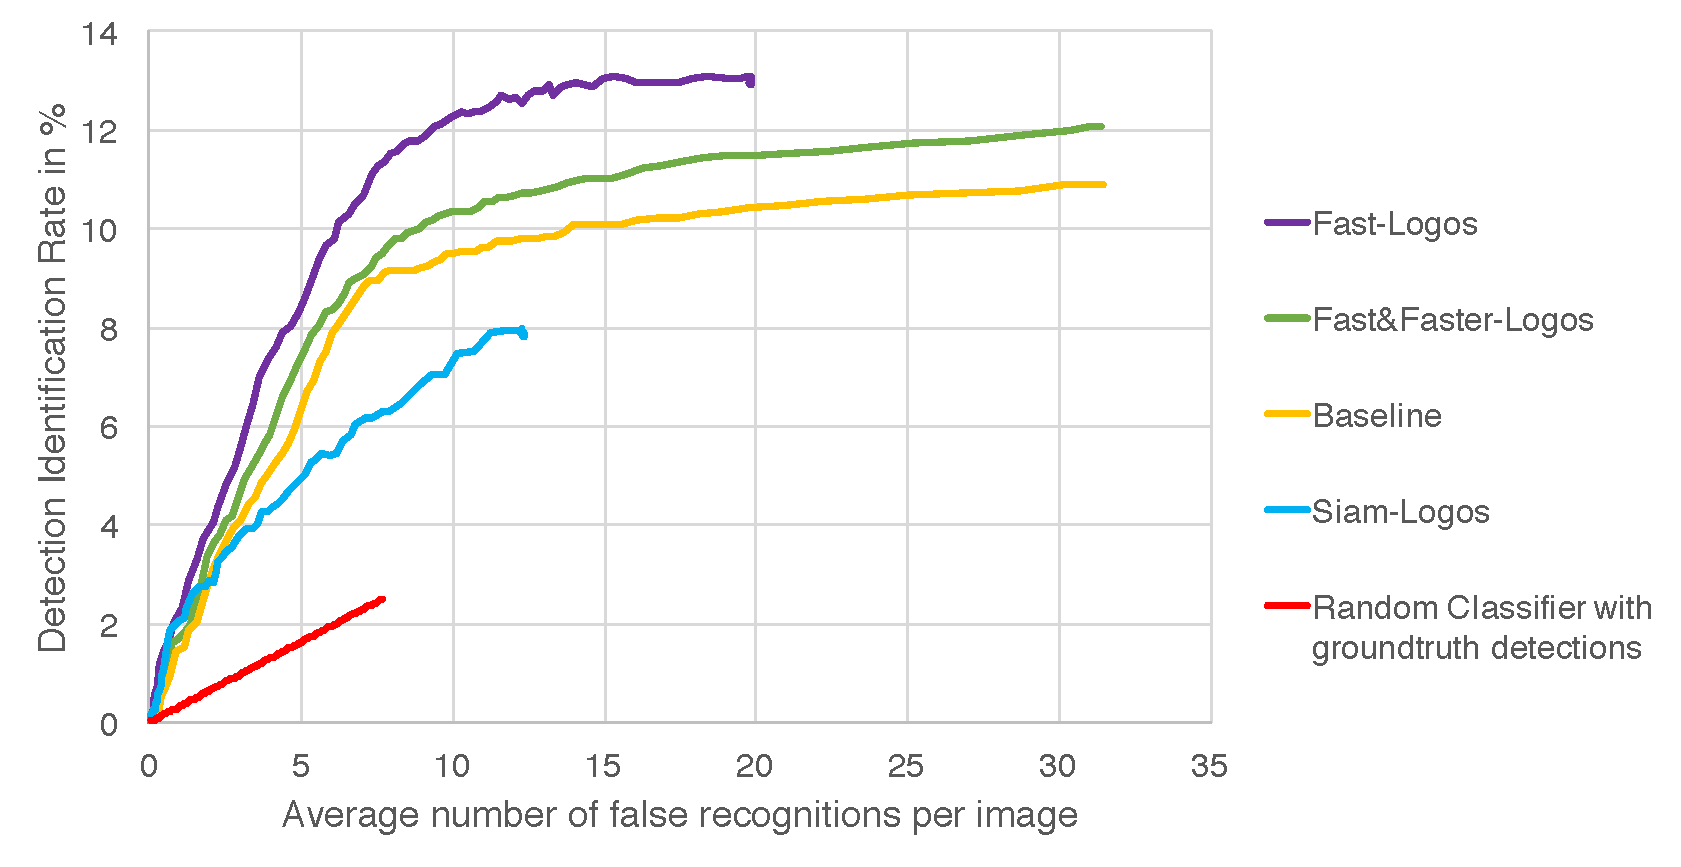
\includegraphics[height=55mm]{eval1} 
	\end{figure}
\end{frame}

\begin{frame}
	\frametitle{Evaluation}
	\heading{R-CNN-Logos vs. Baseline}
	\begin{figure}
	        \centering
       		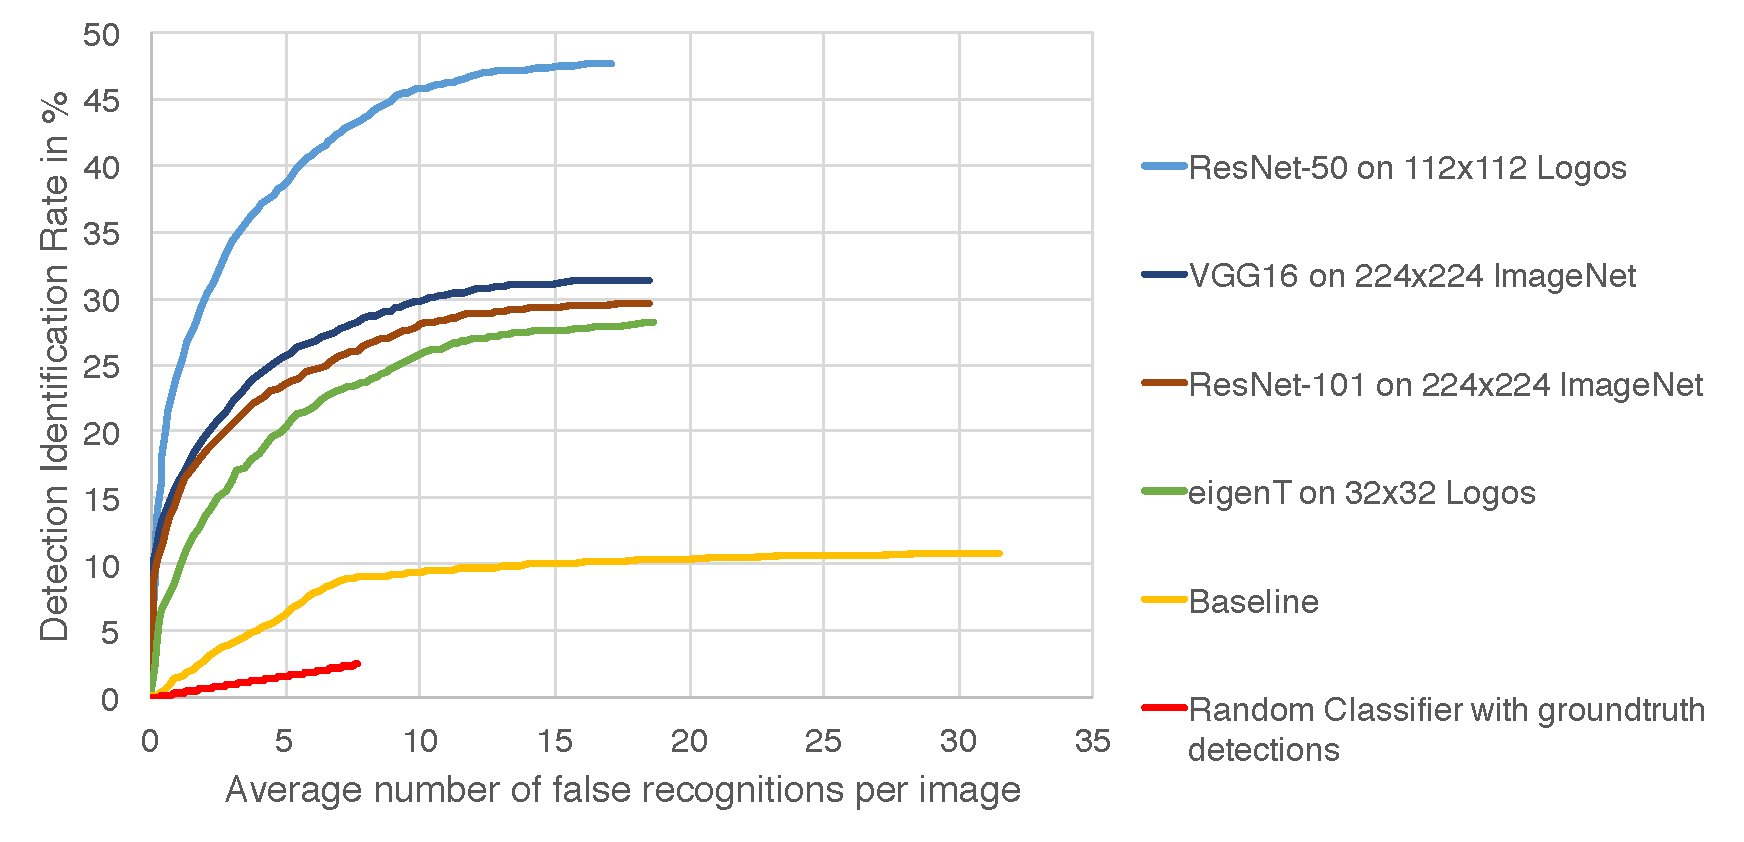
\includegraphics[height=55mm]{eval2} 
	\end{figure}
\end{frame}

\begin{frame}
	\frametitle{Evaluation}
	\heading{Verarbeitungszeit pro Bilder und beste DIR Werte}
	\begin{figure}
	        \centering
       		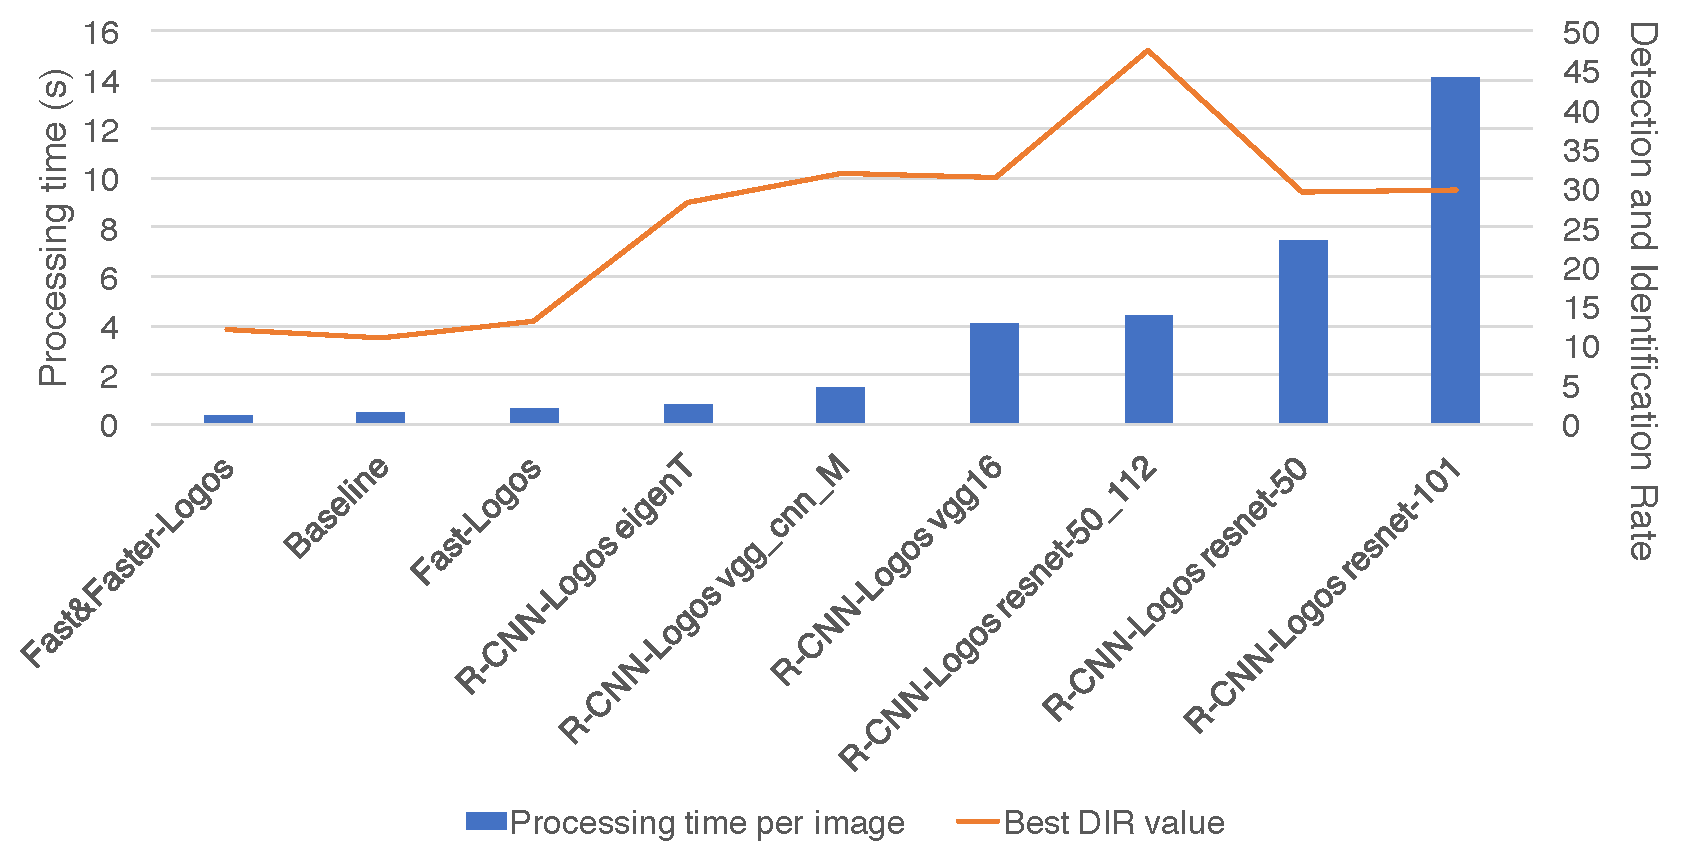
\includegraphics[height=55mm]{timeeval} 
	\end{figure}
\end{frame}

\begin{frame}
	\frametitle{Evaluation}
	\heading{Performance von Klassen, die in dem Training-Set vorkommen}
	\begin{figure}
	        \centering
       		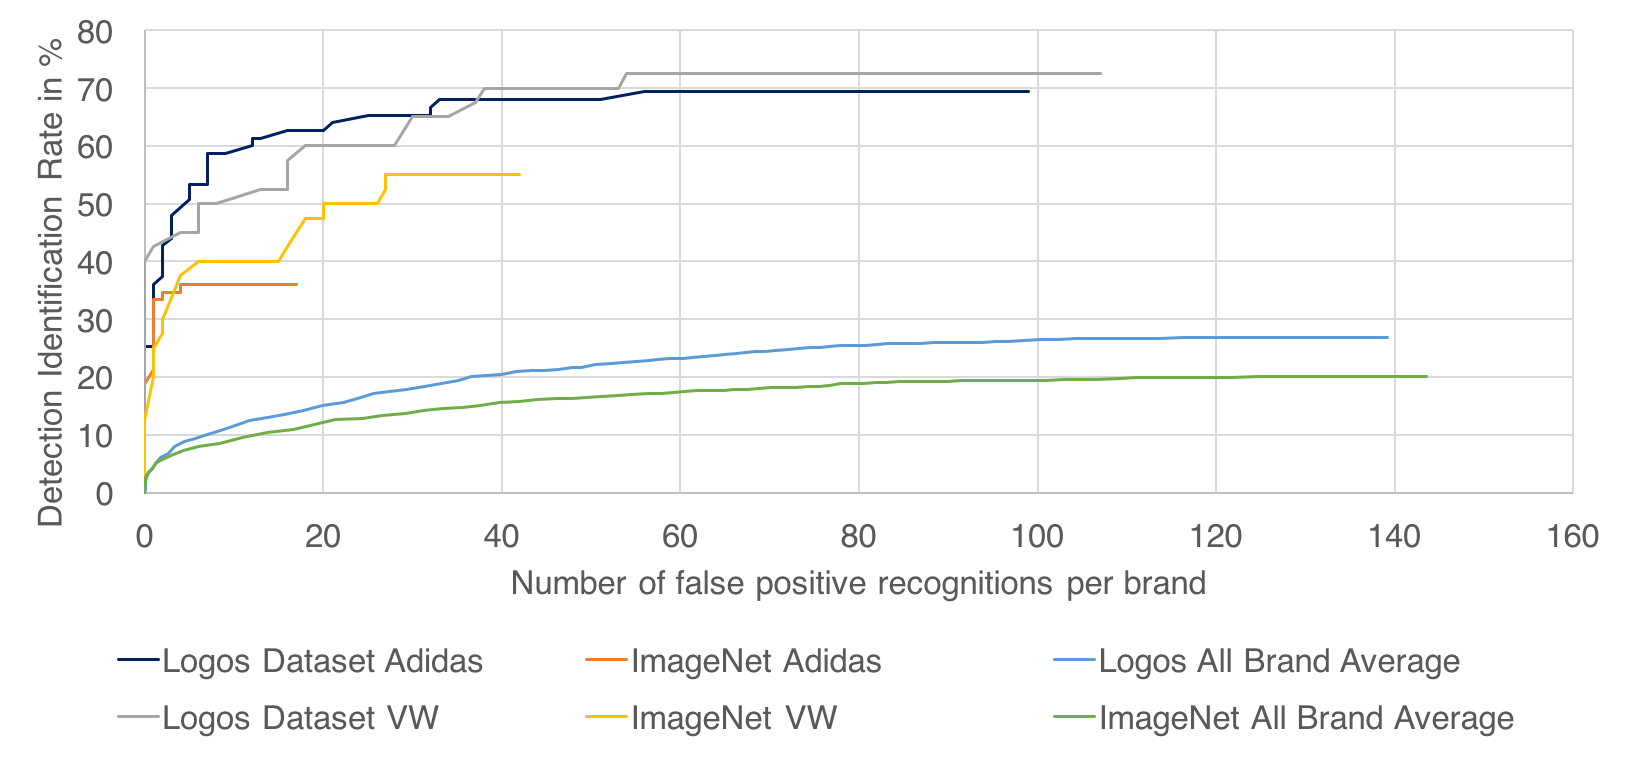
\includegraphics[height=50mm]{commonbrandseffect} 
	\end{figure}
\end{frame}

\begin{frame}
	\frametitle{Evaluation}
	\heading{Logo Vergleich}
	\begin{figure}
	        \centering
       		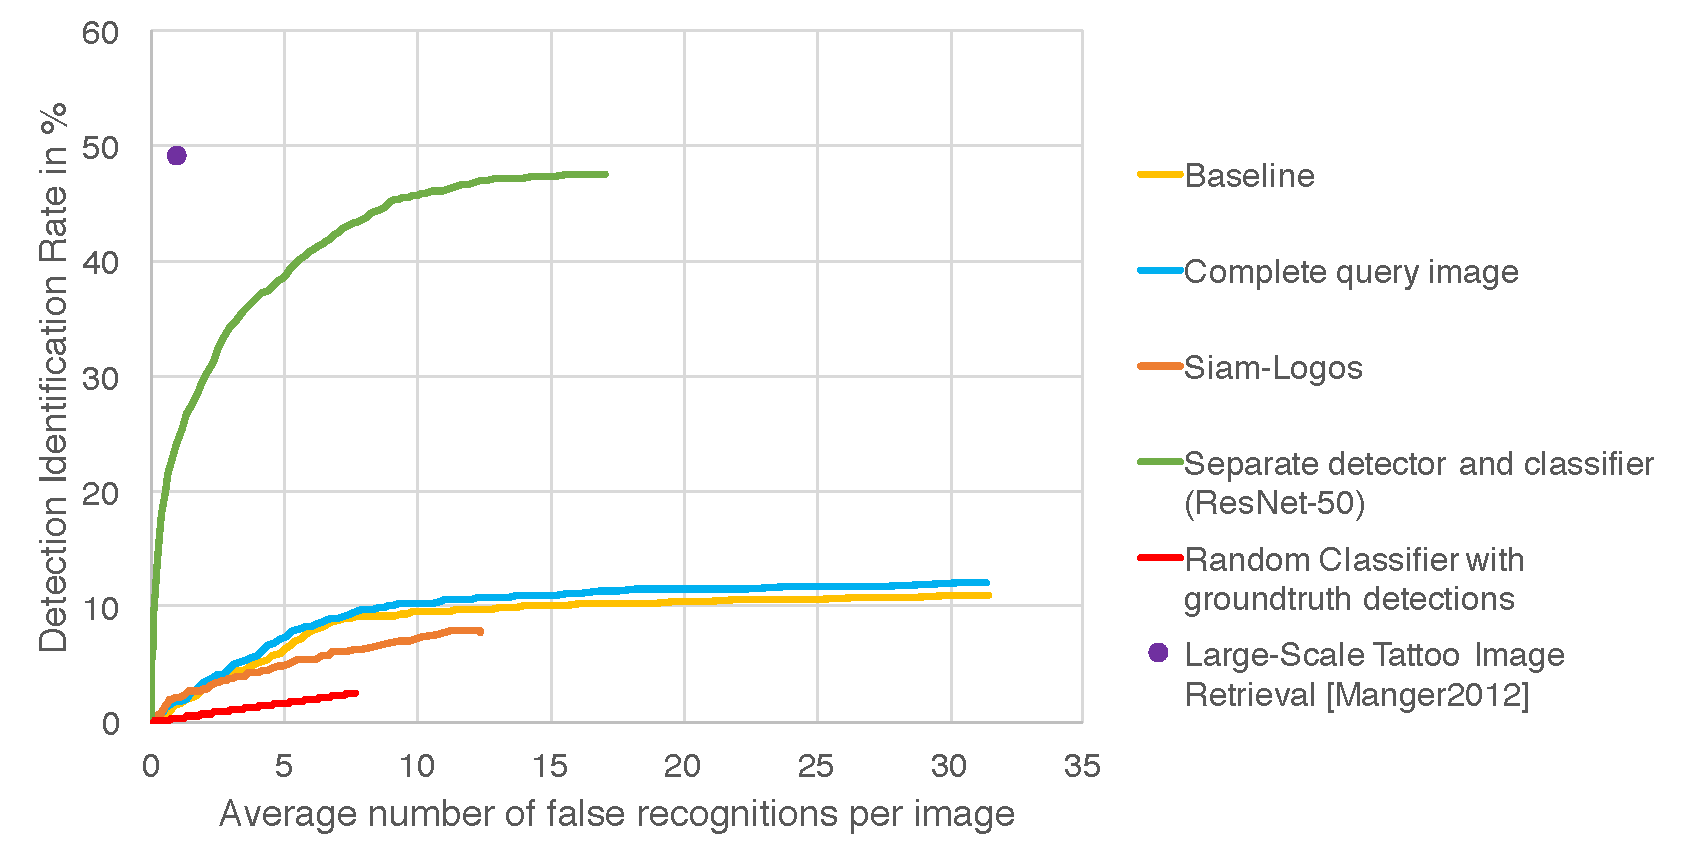
\includegraphics[height=50mm]{clsevalfull} 
	\end{figure}
\end{frame}

\end{document}
